\documentclass[12pt,a4paper,twoside,openany,titlepage,final]{book}

\usepackage[dvips]{geometry}
\geometry{textwidth=15cm,textheight=24cm,top=3.5cm}

\usepackage[small,sf]{caption}

\usepackage{sectsty}
\allsectionsfont{\sffamily\raggedright}

\usepackage{lmodern}
\usepackage[T1]{fontenc}
\usepackage{textcomp}

\usepackage{array}
\extrarowheight4pt

\usepackage{supertabular}

% \usepackage{floatflt}

\usepackage{graphicx}

\usepackage{amsmath}
\usepackage{amssymb}
\usepackage{bm}

\usepackage{multicol}
\premulticols0.0em

\usepackage{fancyhdr}

\pagestyle{fancy}

\bibliographystyle{plain}

\usepackage{makeidx}

\usepackage{color}

\usepackage{subfigure}
\usepackage{wrapfig}
\DeclareGraphicsExtensions{.png, .jpg, .pdf, .eps} 

\definecolor{link_color}{rgb}{0,0,1}
\definecolor{MARK_color}{rgb}{1,0,0}
\definecolor{filename_color}{rgb}{0.6,0.6,0.6}
% This usepackage command MUST BE LAST !!!
% More details on the hyperref package, including an extensive list of global package options
% can be found at http://www.tug.org/applications/hyperref/manual.html
\usepackage[backref           = page,
            colorlinks        = true,
            linkcolor         = link_color,
            menucolor         = link_color,
            citecolor         = link_color,
            urlcolor          = link_color,
            bookmarksnumbered = true,
            hyperindex        = true]{hyperref}
\hypersetup{pdfauthor  = {Volker Blum et al.},
            pdftitle   = {AIMS Manual},
            pdfsubject = {A users manual for the code package FHI-AIMS}}

%\pagestyle{headings}
%\pagenumbering{arabic}

\linespread{1.0}

\newcommand{\la}{$\langle$}
\newcommand{\ra}{$\rangle$}
\newcommand{\boldk}{\mbox{\boldmath$k$}}
\newcommand{\boldr}{\mbox{\boldmath$r$}}
\newcommand{\bolds}{\mbox{\boldmath$\sigma$}}
\newcommand{\boldp}{\mbox{\boldmath$p$}}
\newcommand{\boldR}{\mbox{\boldmath$R$}}
\newcommand{\boldE}{\mbox{\boldmath$E$}}
\newcommand{\boldF}{\mbox{\boldmath$F$}}
\newcommand{\boldG}{\mbox{\boldmath$G$}}
\newcommand{\erf}{\mathop{\mathrm{erf}}}
\newcommand{\erfc}{\mathop{\mathrm{erfc}}}
\newcommand{\bfr}{{\bf r}}
\newcommand{\bfrp}{{\bf r'}}
\newcommand{\bfk}{{\bf k}}
\newcommand{\bfq}{{\bf q}}
\newcommand{\bfR}{{\bf R}}
\newcommand{\bfRp}{{\bf R'}}
\newcommand{\bfRpp}{{\bf R''}}

\renewcommand{\floatpagefraction}{0.75}

% don't like something in the Manual? \MARK{} it and readers will definitely notice!
\newcommand{\MARK}[1]{\textbf{\color{MARK_color} #1}}

\newcommand{\keyword}[1]
{\hyperlink{#1}{\texttt{#1}}}

\newcommand{\subkeyword}[2]{\hyperlink{#1 #2}{\texttt{#2}}}

\newcommand{\option}[1]{\texttt{#1}}


% use this to define a keyword, automatically creates all the links here.
\newcommand{\keydefinition}[3]
{
\centerline{\rule{1.0\textwidth}{1pt}}
\hypertarget{#1}{\textbf{Tag: \texttt{#1}}{ \color{filename_color} (#2)}}
\index{#1@\texttt{#1}}
\\[2ex] \hspace*{0.05\textwidth}
\begin{minipage}{0.92\textwidth}
  #3
\end{minipage} \\
}

\newcommand{\subkeydefinition}[4]
{
\centerline{\rule{1.0\textwidth}{1pt}}
\hypertarget{#1 #2}{\textbf{\keyword{#1} sub-tag: \texttt{#2}} { \color{filename_color} (#3)}}
\index{#1@\texttt{#1}!#2@\texttt{#2}}
\\[2ex] \hspace*{0.05\textwidth}
\begin{minipage}{0.92\textwidth}
  #4
\end{minipage} \\
}

\newcommand{\keydefinitiontwo}[4]
{
\centerline{\rule{1.0\textwidth}{1pt}}
\hypertarget{#1}{\textbf{Tags:\ \texttt{#1}}{ \color{filename_color} (#3)}}
\hypertarget{#2}{\textbf{\newline\phantom{Tags:}\ \texttt{#2}\phantom{a}}{ \color{filename_color} (#3)}}
\index{#1@\texttt{#1}}
\index{#2@\texttt{#2}}
\\[2ex] \hspace*{0.05\textwidth}
\begin{minipage}{0.92\textwidth}
  #4
\end{minipage} \\
}

\newcommand{\keydefinitionthree}[5]
{
\centerline{\rule{1.0\textwidth}{1pt}}
\hypertarget{#1}{\textbf{Tags:\ \texttt{#1}}{ \color{filename_color} (#4)}}
\hypertarget{#2}{\textbf{\newline\phantom{Tags:}\ \texttt{#2}}{ \color{filename_color} (#4)}}
\hypertarget{#3}{\textbf{\newline\phantom{Tags:}\ \texttt{#3}}{ \color{filename_color} (#4)}}
\index{#1@\texttt{#1}}
\index{#2@\texttt{#2}}
\index{#3@\texttt{#3}}
\\[2ex] \hspace*{0.05\textwidth}
\begin{minipage}{0.92\textwidth}
  #5
\end{minipage} \\
}


\makeindex

\begin{document}

\fancyhf{}
\fancyhead[LO]{\sffamily\slshape \nouppercase{\rightmark}}
\fancyhead[RE]{\sffamily\slshape \nouppercase{\leftmark}}
\fancyhead[LE,RO]{\sffamily \thepage}
\fancypagestyle{plain}{
  \fancyhf{}
  \fancyhead[LE,RO]{\sffamily \thepage}
  \renewcommand{\headrulewidth}{0pt}
                      }
\renewcommand{\linespread}{1.0}

\parindent0.0ex
\parskip1.3ex

%\renewcommand{\baselinestretch}{1.0}

\sffamily

\thispagestyle{empty}
\vspace*{-2.0cm}

\begin{center} \huge
\centerline{\rule{1.0\textwidth}{1pt}}

\textbf{Fritz Haber Institute \\ \emph{ab initio} molecular
       simulations: FHI-aims}

\centerline{\rule{1.0\textwidth}{1pt}}

\vspace*{0.5cm}

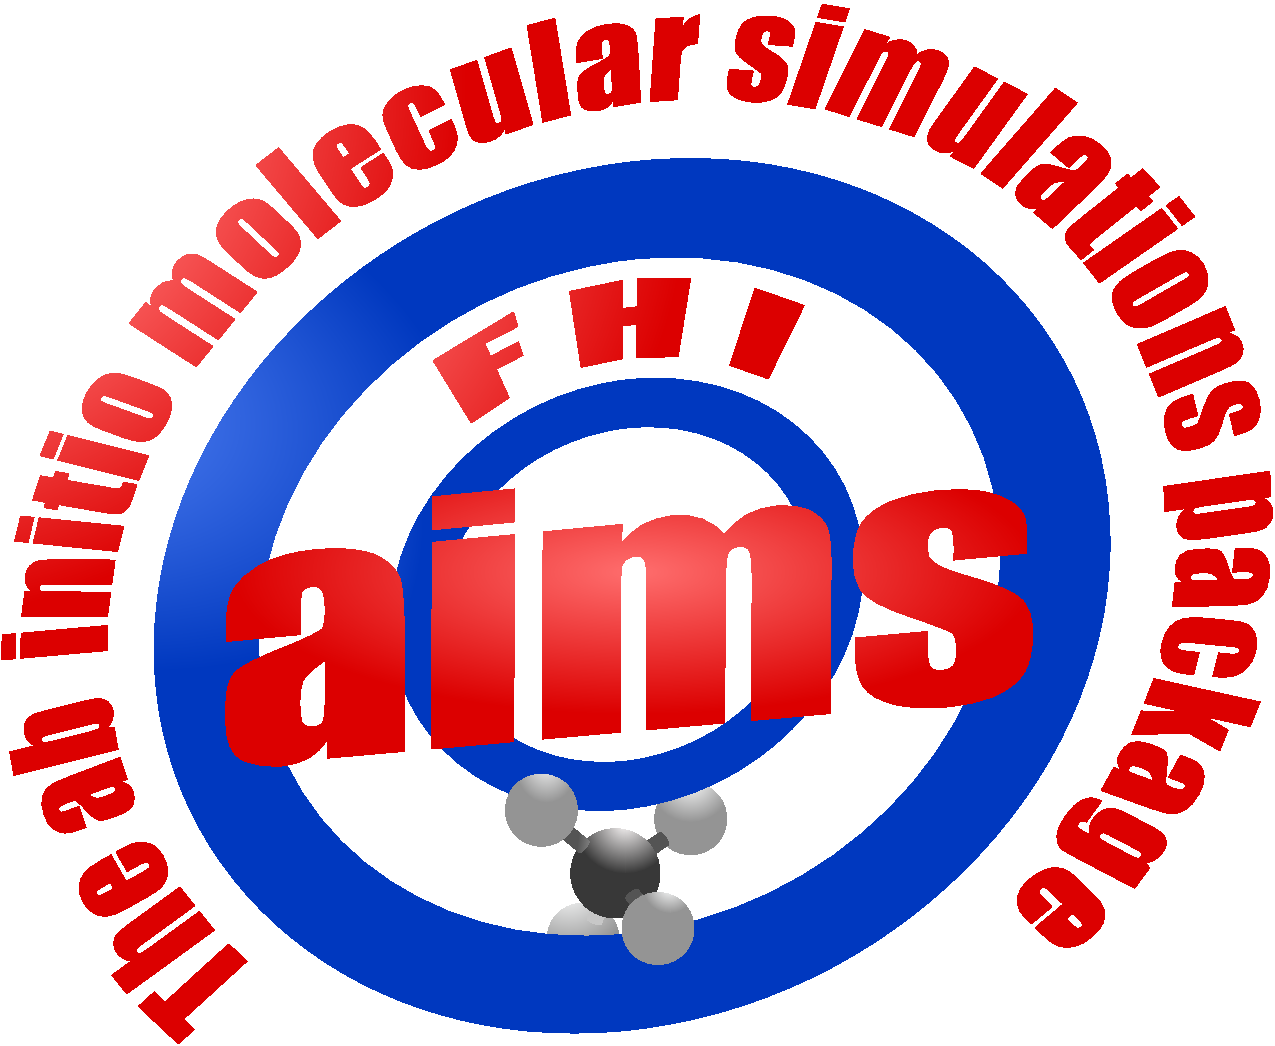
\includegraphics[width=0.7\textwidth]{aims_logo}

\vspace*{0.5cm}

\LARGE {All-Electron Electronic Structure Theory \\ with Numeric Atom-Centered
  Basis Functions \\[3.0cm] A Users' Guide}
\end{center}

\vspace*{0.0cm}

\centerline{\rule{1.0\textwidth}{1pt}}
\begin{center} \large
     FHI-aims team
     \\      Fritz-Haber-Institut der Max-Planck-Gesellschaft,
     Berlin \\
     and many contributors around the world. \\
\today
\end{center}

\newpage

\tableofcontents

%\chapter[The AITRANSS package]{The {\LARGE AITRANSS} package}
%\label{Ch:aitranss}

%The \textsc{aitranss} ({\it ab initio} transport simulations) package is 
%a project under continuous development at the Institute of Nanotechnology 
%of the Karlsruhe Institute of Technology (KIT), Germany, since 2002. In 
%brief, when combined with FHI-aims, \textsc{aitranss} provides a 
%post-processor module that enables, e.g., calculation of the electron 
%transport characteristics of molecular junctions based on a Landauer 
%formalism in a (non-equilibrium) Green's function formulation.

%Currently, the version of the code accessible to FHI-aims users is
%limited to computation of the ballistic (Landauer-B\"uttiker) transmission
%function and partial atom-projected density of states. 
%According to current planning advanced options, e.g., out of
%equilibrium transport response, will be available in the future releases.

%A discussion of the underlying physical formalism and details of the
%implementation are described in the references \cite{Arnold2007,Wilhelm2013,Bagrets2013}:

%\begin{center}
%\parbox[c]{0.85\textwidth}
%{\small
%A.\ Arnold, F.\ Weigend, and F.\ Evers,
%"Quantum chemistry calculations for molecules coupled to reservoirs:
%Formalism, implementation, and application to benzenedithiol."
%J.\ Chem.\ Phys.\ \textbf{126}, 174101 (2007).
%}
%\medskip

%\parbox[c]{0.85\textwidth}
%{\small
%J.\ Wilhelm, M.\ Walz, M.\ Stendel, A.\ Bagrets, and F.\ Evers,
%"Ab initio simulations of scanning-tunneling-microscope
%images with embedding techniques and application to C58-dimers 
%on Au(111)." Phys.\ Chem.\ Chem.\ Phys.\ \textbf{15}, 6684 (2013).
%}
%\medskip

%\parbox[c]{0.85\textwidth}
%{\small
%A.\ Bagrets, "Spin-polarized electron transport across metal-organic 
%molecules: a density functional theory approach." 
%J.\ Chem.\ Theory Comput.\ \textbf{9}, 2801 (2013).
%}
%\medskip

%\end{center}

%Please, cite the above works together with 
%FHI-aims publications, when using \textsc{aitranss}.

%For questions and bug reports, contact
%Alexej Bagrets (\verb,Alexej.Bagrets@kit.edu,).

%% Chapter: aitranss module

%%%%%%%%%%%%%%%%%%%%%%%%%%%%%%%%%%%%%%%%%%%%%%%%%%%%%%%%%%%%%%%%%%%%%%%
\section{Source code and supporting materials} 
\label{sec:aitranss:source}

The source code and supporting material of the \textsc{aitranss}-module
for the FHI-aims package is placed in the subdirectory \verb,aitranss/,.
This directory contains subdirectories:

\begin{itemize}
 \item \verb,source/, : with the Fortran90 code and the example
   \verb,Makefile, ; 
 \item \verb,tcontrol.script/, : contains a script
 \verb,tcontrol.aims.x,,
   which is served to prepare a mandatory input file \verb,tcontrol,
   for the transport-type calculation ;
 \item \verb,electrodes.library/, : contains a library of representative
   gold (Au) clusters
   (xyz-files) which should be linked, via anchoring groups, to your
   molecular system to create an ``extended molecule'': its electronic
   structure (Kohn-Sham molecular orbitals and energies) is a prerequisite
   to compute transport characteristics ;
 \item \verb,examples/, : contains examples, with input and output
   files of the FHI-aims and \textsc{aitranss}; \verb,README, files
   found in this subdirectory contain also short guidelines on how an
   input for a particular transport calculation has been created.
\end{itemize}

\section[Compiling the \textsc{aitranss} module]%
{Compiling the {\large AITRANSS} module}
\label{sec:aitranss:compiling}

Please, use a template of the \verb,Makefile, found in the directory
\verb,source/,, and adjust variables referring to compiler (\verb,FC,
and \verb,LD,), compiler's options (\verb,FLAGS,) and a path to libraries
(\verb,LIBS,) at your computer system.  A mandatory prerequisite to build 
the code is a Fortran 90/95 capable compiler and a compiled version of 
{\small{LAPACK}} and {\small{BLAS}} (for example, Intel's {\small{MKL}}). 
A~binary (\verb,aitranss.x,) built by the \verb,Makefile, will go to the 
\verb,bin/, directory of the FHI-aims.

In contrast to FHI-aims, the current release of \textsc{aitranss}
is not yet based on MPI. However, you are encouraged to use a fortran
compiler option(s), aka \verb,"-openmp", and \verb,"-O2", for Intel's
\verb,ifort,,\ to enable the auto-parallelizer to build a multithreaded
code based on OpenMP directives.

According to our experience, a generated code can be safely executed in
parallel within a single compute node with multiple processors, and with
a significant gain in computation time.

We advise you as well to copy a script \verb,tcontrol.aims.x, found
in the directory \linebreak \verb,tcontrol.script/, to the directory
\verb,bin/, of the FHI-aims installation, and to make files in that
directory accessible for the execution from a command line by adjusting
your shell variable \verb,PATH,.

\clearpage

%%%%%%%%%%%%%%%%%%%%%%%%%%%%%%%%%%%%%%%%%%%%%%%%%%%%%%%%%%%%%%
\section{How to set-up and run transport calculations}
%%%%%%%%%%%%%%%%%%%%%%%%%%%%%%%%%%%%%%%%%%%%%%%%%%%%%%%%%%%%%%
\label{sec:aitranss:howto}

\subsection{FHI-aims run: input and output} 
\label{subsec:fhiaims}

Having your molecule "at hands", use your favorite modeling and
visualization tools/\-software, and prepare an extended structure
by linking the molecule via anchoring groups to two atomic clusters,
representing parts of macroscopic \textit{source} and \textit{drain}
electrodes.  Consult the \verb,electrodes.library/, directory, and
use predefined Au clusters found there.  A typical example of an
``extended molecule'', which you are requested to build, is shown in
Fig.~\ref{fig:extended_molecule}.

Include a line

\noindent
\phantom{xxx}\keyword{output}\ \subkeyword{output}{aitranss}
%\begin{verbatim}
%   output aitranss
%\end{verbatim}

\noindent
into your \verb,control.in, file. Furthermore, following settings are
recommended for the self-consistent DFT calculation:

\begin{verbatim}
  occupation_type    gaussian 0.1
  mixer              pulay
    n_max_pulay        10
    charge_mix_param   0.2

  sc_accuracy_rho    1E-4
  sc_accuracy_eev    1E-2
  sc_accuracy_etot   1E-6

  relativistic zora scalar 1.0e-10
\end{verbatim}

Invoke FHI-aims exploiting a cluster type (non-periodic)
calculation. After the FHI-aims run is finished, you'll find in your
directory three ASCII files: \verb,basis-indices.out,, \verb,omat.aims,
and \verb,mos.aims,. These files contain: some limited information on
basis functions; overlap integrals; and data on Kohn-Sham molecular
orbitals \& energies of the ``extended molecule'', respectively. If
spin channels of your system are not identical, \verb,mos.aims,
will be substituted by two other files called \verb,alpha.aims, and
\verb,beta.aims,.

\subsection[What to be aware of before running \textsc{aitranss} module]%
{What to be aware of before running {\normalsize AITRANSS} module} 
\label{subsec:aitranss:whattobeaware}

The \textsc{aitranss} module should be run from the same directory,
where output files of FHI-aims are placed.  A file \verb,geometry.in,
is mandatory and should also be there.

A file \verb,control.in, is not used. Instead, another mandatory file for
the transport calculation is \verb,tcontrol,.  Please, \textit{always} use
a script \verb,tcontrol.aims.x, to create this file.  Executing a script
\verb,tcontrol.aims.x, without arguments outputs a help information:

\clearpage

\begin{verbatim}
[...]
--------------------------------------------------------------
"tcontrol.aims.x"   script creates a mandatory file "tcontrol"
                    which is required to run the "aitranss"
                    post-processing module after FHI-aims
--------------------------------------------------------------
USAGE: tcontrol.aims.x [ -option <argument> ] ...

where options & arguments are:

                       ! electrodes geometry:
 -lsurc <atom1>        three atoms which define an outermost
 -lsurx <atom2>        LEFT surface layer of the extended
 -lsury <atom3>        molecule

 -rsurc <atom4>        three atoms which define an outermost
 -rsurx <atom5>        RIGHT surface layer of the extended
 -rsury <atom6>        molecule

 -nlayers <number>     number of atomic layers coupled to 
                       reservoirs via a self-energy

                       ! energy window, in Hartree [H], to
                       ! output transmission function T(E) :
 -ener  <E1[H]>        initial energy point, E1
 -estep <dE[H]>        energy step, dE
 -eend  <E2[H]>        final energy point, E2

                       ! output :
 -outfile <file_name>  output file name for T(E) [default: TE.dat]

\end{verbatim}

When executed with options and arguments, a script \verb,tcontrol.aims.x,
checks for the \verb,geometry.in, file and other mandatory FHI-aims
output files (\verb,basis-indices.out,, \verb,omat.aims,, \verb,mos.aims,
or \verb,alpha.aims, \& \verb,beta.aims,) in your directory, reads from
these files information on a system size and the Hamiltonian $H$ and
overlap matrix dimension, and exports this information together with
your arguments to an ASCII file \verb,tcontrol,. Options and arguments
are used: (i) to provide information on the self-energy construction;
(ii) to introduce an energy window for the calculation of the transmission
function $T(E)$, and (iii) (optionally) to introduce an output file name
for $T(E)$.

\begin{figure} 
\centering
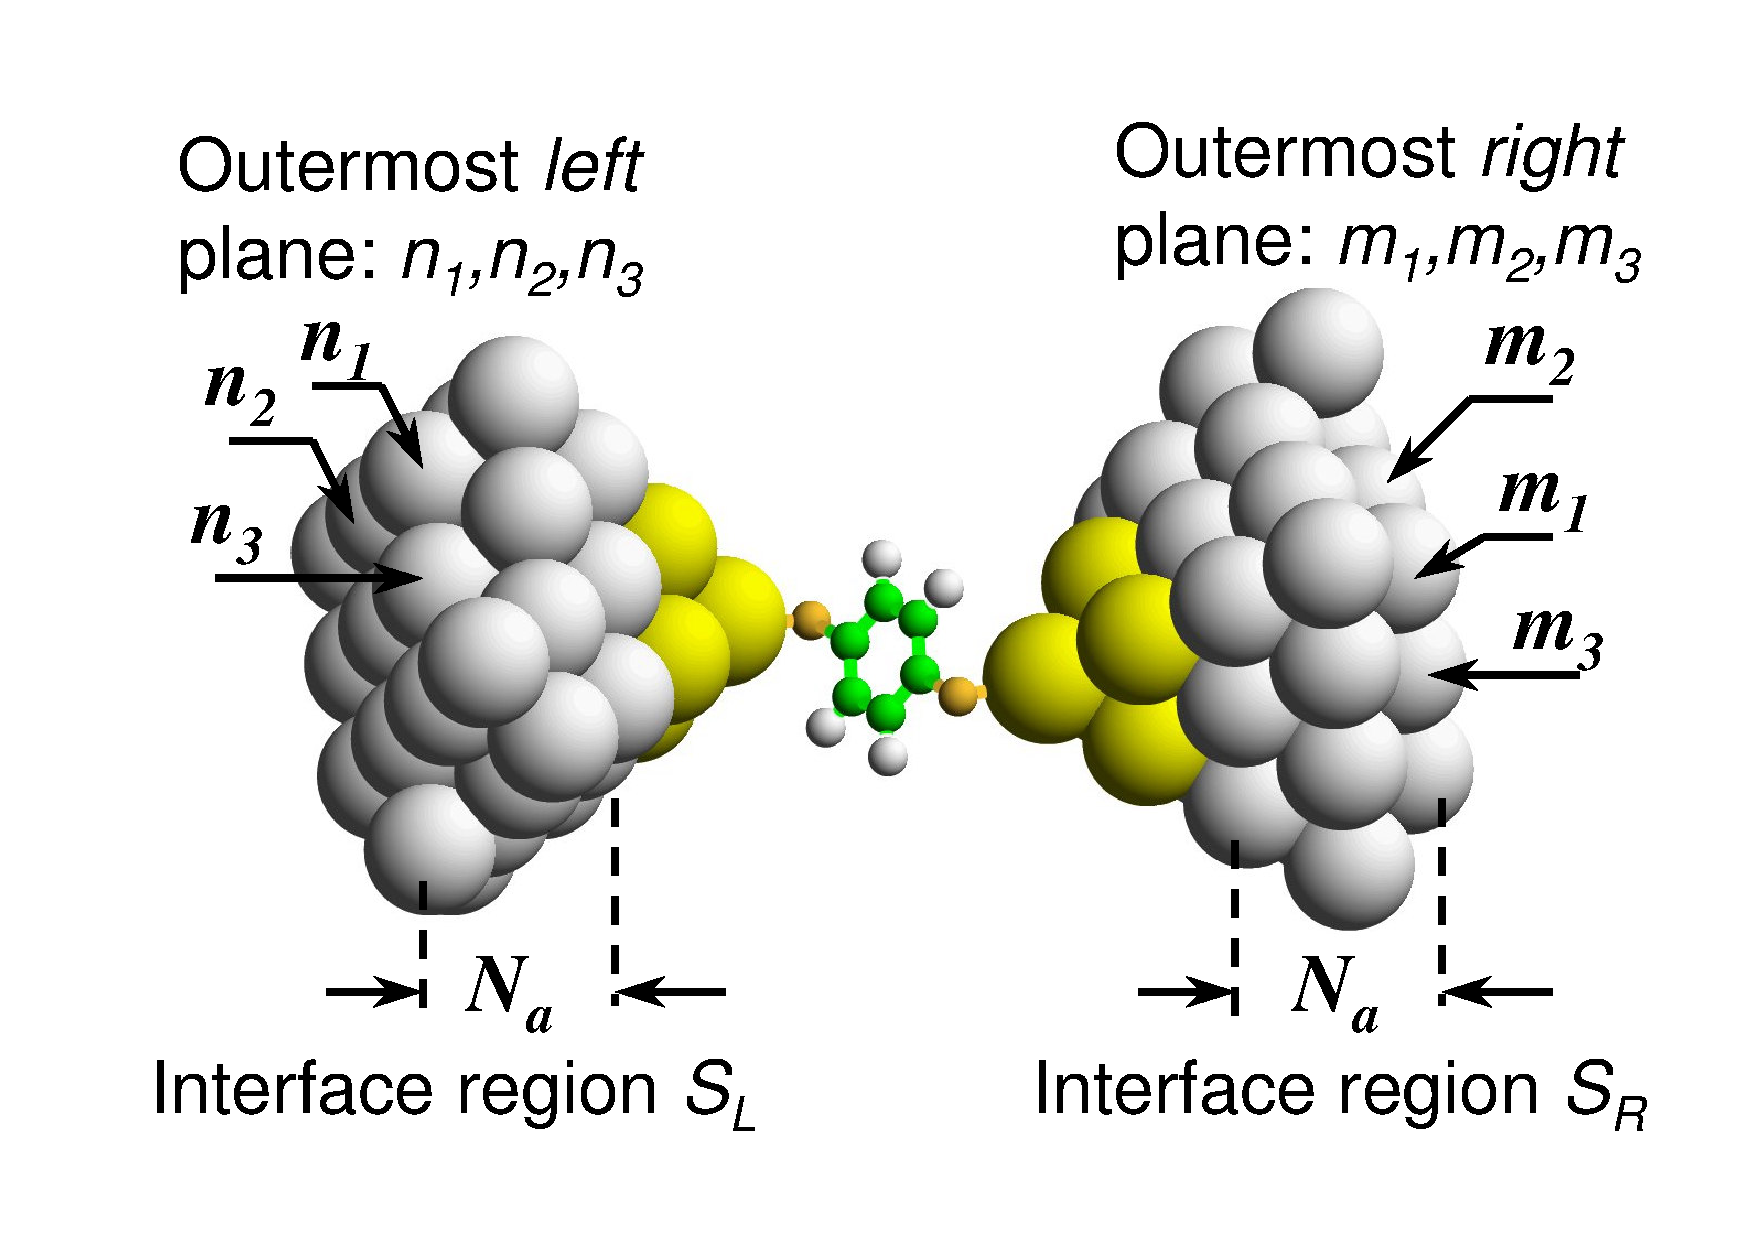
\includegraphics[width=0.6\textwidth]{fig_extended_molecule.pdf}
\caption{% 
\label{fig:extended_molecule} A schematic view of the
``extended molecule''.  The shaded regions are interfaces to the two
reservoirs. Within the interface regions absorbing boundary conditions
are active and the self-energy $\Sigma$ is introduced. A user defines
interface regions by specifying the outermost \textit{left} and
\textit{right} atomic planes (introducing indices of three different atoms
that form a triangle, $n_1,n_2,n_3$, and $m_1,m_2,m_3$, respectively)
and the amount of atomic layers, $N_a$.  } 
\end{figure}

\emph{Comment on the self-energy}. When an ``extended molecule''
is contacted to macroscopic reservoirs, a propagation of an electron
with energy $E$ within a subspace limited by the ``extended molecule''
is described by the Green's function: $ G^{-1}(E) = E - H - \Sigma(E)
$, where a self-energy $\Sigma(E)$ accounts for the interaction
between a finite system and macroscopic reservoirs.  As argued in
Refs.~\cite{Arnold2007,Evers2006}, if atomic clusters introduced to model parts
of metallic electrodes are large enough, the reservoirs can be modeled
by absorbing boundary conditions which become active at the interface
regions ${\cal S}_L$ and ${\cal S}_R$ (labeled by a gray color in
Fig.~\ref{fig:extended_molecule}) where the ``extended molecule'' is
coupled to reservoirs. Within this model, the self-energy is approximated
by an energy-independent, diagonal matrix, 
\[
 \Sigma^{\mu\mu'}_{nn'} \approx - i \eta_n \delta_{nn'}\delta_{\mu\mu'},
\] 
where indices $n$ and $n'$ label atoms, and $\mu$ and $\mu'$ label
corresponding internal degrees of freedom (i.e., atom-centered basis
functions). Here absorption rates $\eta_n$ are allowed to have non-zero
weights only within the interface regions ${\cal S}_L$ and ${\cal S}_R$.
A user defines interface regions by specifying the outermost \textit{left}
and \textit{right} atomic planes (introducing indices of three different
atoms forming a triangle, $n_1,n_2,n_3$, and $m_1,m_2,m_3$, respectively)
and the amount of atomic layers, $N_a$.  
%{\bf AB: Is the number of layers for left and right hand side the same?}

\subsection{% 
How to create a mandatory file \texttt{tcontrol}}
\label{subsec:aitranss:tcontrol}

To create a \verb,tcontrol, file, a \verb,tcontrol.aims.x, script should
be launched with the following options and arguments:

\verb,tcontrol.aims.x, 
\verb,-lsurc, $n_1$ 
\verb,-lsurx, $n_2$
\verb,-lsury, $n_3$ 
\verb,-rsurc, $m_1$ 
\verb,-rsurx, $m_2$ 
\verb,-rsury, $m_3$ 
\verb,-nlayers, $N_a$ 
\verb,-ener, $E_1$ 
\verb,-estep, $dE$
\verb,-eend, $E_2$

\begin{itemize}

\item where integer numbers $n_1$, $n_2$, $n_3$ are indices of three
 different atoms fixing the outermost \textit{left} atomic plane of the
 ``extended molecule'' (see Fig.~\ref{fig:extended_molecule}); atoms are
 numbered according to their appearance in file \verb,geometry.in, ;

\item integer numbers $m_1$, $m_2$, $m_3$ are indices of three different
 atoms fixing the outermost \textit{right} atomic plane of the ``extended 
 molecule'' (see Fig.~~\ref{fig:extended_molecule});

\item an integer $N_a$ indicates the number of atomic layers
 defining the interface regions ${\cal S}_L$ and ${\cal S}_R$  (see
 Fig.~\ref{fig:extended_molecule}); users are strongly advised to take Au
 clusters of similar size from the directory \verb,electrodes.library/, and
 use a parameter $N_a$ suggested in the header of a library file.  Using Au
 clusters of similar size insures that $N_a$ can be consistently chosen to
 be the same for both \textit{left} and \textit{right} interface regions;

\item real numbers $E_1$, $E_2$ and a positive real number $dE$ define the
 energy window $[E_1,E_2]$ and energy step $dE$ to calculate transmission
 function $T(E)$;

\item optionally, you can launch the script with "\verb,-output,
 \textit{filename}" where \textit{filename} is a string, specifying a
 name of the output file for $T(E)$.  
\end{itemize}
 
An example of the transport calculation set-up for the
Au-benzene-dithiol-Au\ junction can be found in the directory
\texttt{examples/au-c6h6-au/}.  A script \texttt{tcontrol.aims.x} has
been executed there with the following options and arguments:

\begin{verbatim} 
tcontrol.aims.x -lsurc 34 -lsurx 30 -lsury 36 -rsurc 35 -rsurx 33
 -rsury 31 -nlayers 2 -ener -0.4000 -estep 0.0001 -eend 0.0000
\end{verbatim}

to create the following file \verb,tcontrol,:

\begin{verbatim}
#input data for the aitranss module
$aims_input on
$landauer on
$coord   file=geometry.in
$natoms  50
$basis   file=basis-indices.out
$read_omat file=omat.aims
$scfmo   file=mos.aims
$nsaos   2268
$ecp     on
$lsurc   34
$lsurx   30
$lsury   36
$rsurc   35
$rsurx   33
$rsury   31
$nlayers 2
$s1i     0.1d0
$s2i     0.05d0
$s3i     0.025d0
$ener   -0.4000
$estep   0.0001
$eend    0.0000
$output  file=TE.dat
$testing off
$end
\end{verbatim}

Detailed description of keywords in file  \verb,tcontrol, are given in
the paragraph~\ref{sec:aitranss:keywords}.

%%%%%%%%%%%%%%%%%%%%%%%%%%%%%%%%%%%%%%%%%%%%%%%%%%%%%%%%%%%%%
\subsection{% 
How to submit a transport calculation and its output} 
\label{subsec:aitranss:calc}
%%%%%%%%%%%%%%%%%%%%%%%%%%%%%%%%%%%%%%%%%%%%%%%%%%%%%%%%%%%%%

Assuming a binary file \verb,aitranss.x, is placed\ in the directory
\verb,bin/, of the FHI-aims installation\ which is referenced in your
shell variable \verb,PATH,, you can run the transport type calculation
from a command line, like

\verb,> aitranss.x | tee my.transport.calc.out,

or

\verb,> nohup aitranss.x > my.transport.calc.out &,

FHI-aims output files together with information provided from files
\verb,tcontrol, and \linebreak \verb,geometry.in, will be used by the
\textsc{aitranss} module to reconstruct a Kohn-Sham Hamiltonian ($H$) of the
``extended molecule'', to supplement $H$ with the self-energy $\Sigma$,
and to compute a ballistic (Landauer-B\"uttiker) transmission function,
exploiting Green's function formalism.

After calculation is finished, you'll get two files. The first file with
a default name \verb,TE.dat, contains information on the transmission
function, $T(E)$. Data in this file are arranged in columns as indicated
in a file's header: (i) first column is energy in Hartree (atomic) units;
(ii) second column is energy in eV units given with respect to the Fermi
energy, which is also stated in the file's header; (iii) third column
contains data on ballistic transmission per spin. If spin channels of
your system are different, there will be present third and forth columns,
referring to transmission in up-spin ($\alpha$) channel and down-spin 
($\beta$) channel, respectively. A contribution to conductance due to 
spin $\sigma$ electrons is given by transmission at the Fermi
energy, $T_{\sigma}(E_F)$, in units $e^2/h$.

The second file has a name \verb,self.energy.in,, and contains information
about the model self-energy construction. A format of this file is similar
to the format of \verb,geometry.in,, where each line corresponds to one
atom in the structure, and atom's specific data are arranged in columns:
(i) columns from 1st till 5th are atom index $n$, its $x$, $y$ and
$z$-coordinates (in~\AA), and atomic symbol, respectively; (ii) 6th column
can contain entries \verb,left,, \verb,right, or \verb,empty,, depending
on whether a given atom $n$ is a part of the left interface region ${\cal
S}_L$, right interface region ${\cal S}_R$, or does not belong to none
of them (see Fig.~\ref{fig:extended_molecule} for details);  (iii) last
column contains a real number in a ``double precision'' \verb,fortan,-like
format: this number is a local leakage rate $\eta_n$, in Hartree units,
at given atom $n$ (for details, please see a comment on the model
self-energy construction, section~\ref{subsec:aitranss:whattobeaware}).

Default leakage rates $\eta_n$'s, used for construction of the
model self-energy, have extensively been tested in numerous previous
transport studies with Au-electrodes.  These rates are referenced
also in the \verb,tcontrol, file and controlled by the keywords (tags)
\keyword{\$s1i}, \keyword{\$s2i} and \keyword{\$s3i} as explained in
detail in the following paragraph~\ref{sec:aitranss:keywords}.

\textcolor{blue}{\emph{Warning: If you are not a transport-expert user
and employ the \textsc{aitranss} module as a ``black-box'' for routine
transport calculations, we advise you against modifying the default
parameters.  This may easily lead to misleading or even completely
incorrect results. } }

If the post-processor transport calculation is resubmitted, a
previously created file \linebreak \verb,self.energy.in, will be
used to initialize the self-energy matrix, as controlled by the 
keyword \keyword{\$self\_energy} in file \verb,tcontrol,,
see section~\ref{sec:aitranss:keywords}.

%%%%%%%%%%%%%%%%%%%%%%%%%%%%%%%%%%%%%%%%%%%%%%%%%%%%%%%%%%%%%
\subsection{% 
Further option: local density of states} 
\label{subsec:aitranss:ldos}
%%%%%%%%%%%%%%%%%%%%%%%%%%%%%%%%%%%%%%%%%%%%%%%%%%%%%%%%%%%%%

Besides a calculation of the ballistic transmission function, you may use \textsc{aitranss}
to output local density of states projected on groups of atoms forming a molecular junction.
This option is controlled by a keyword  \keyword{\$ldos} and described in detail
in the subsequent section ~\ref{sec:aitranss:keywords}.

\section{Keywords of file \texttt{tcontrol}} 
\label{sec:aitranss:keywords}

All keywords (tags) of \texttt{tcontrol} file begin with a special symbol
\verb,$,. Lines starting from~\verb,#, are comment lines.  All lines
after a keyword \keyword{\$end} are ignored.

%%%%%%%%%%%%%%%%%%%%%%%%%%%%%%%%%%%%%%%%%%%%%%%%%%%%%%%%%%%%%%%%%
\keydefinition{\$aims\_input}{tcontrol} 
{
 \noindent 
 Usage:    \keyword{\$aims\_input} \option{on} \\[1.0ex]
 Purpose:  mandatory flag, sets up the FHI-aims like format of
           input/output files. \\
} 

%%%%%%%%%%%%%%%%%%%%%%%%%%%%%%%%%%%%%%%%%%%%%%%%%%%%%%%%%%%%%%%%%

\keydefinition{\$landauer}{tcontrol} 
{
 \noindent 
 Usage: \keyword{\$landauer}\quad \option{flag} \\[1.0ex] 
 Purpose: mandatory keyword; \option{flag} should take values either \texttt{on} or \texttt{off}. 
 If \option{flag} is \texttt{on}, ballistic transmission function is computed. 
 If \option{flag} is \texttt{off}, calculation of the transmission function is not performed. 
 In this case you, however, may wish to compute atom projected local density of states that 
 is controlled by the keyword \keyword{\$ldos}.  \\
}
%%%%%%%%%%%%%%%%%%%%%%%%%%%%%%%%%%%%%%%%%%%%%%%%%%%%%%%%%%%%%%%%%


%%%%%%%%%%%%%%%%%%%%%%%%%%%%%%%%%%%%%%%%%%%%%%%%%%%%%%%%%%%%%%%%%

\keydefinition{\$ldos}{tcontrol} 
{
 \noindent 
 Usage: \keyword{\$ldos}\quad \option{flag} \\[1.0ex] 
 Purpose: optional keyword; \option{flag} can take values \texttt{on} or \texttt{off}. 
 If \option{flag} is \texttt{on}, atom projected local density of states (LDoS) is computed; 
 otherwise (\option{flag} is \texttt{off}) calculation of LDOS is not performed. \\
}
On output, the (energy dependent) density of states of the system is projected onto
atomic orbitals of atoms marked by the same chemical symbols and 
is redirected to corresponding files, which have the self-explanatory names, e.g.
\texttt{ldos.au.dat}, \texttt{ldos.c.dat}, \texttt{ldos.h.dat} and \texttt{ldos.s.dat} 
in the case of benzene-dithiol molecular junction shown in Fig.~\ref{fig:extended_molecule}.
For example, the file \texttt{ldos.c.dat} would contain LDoS summed up over all six C atoms of the molecule.
Furthermore, only LDoS projected onto those electrodes' atoms of the ``extended molecule'' which are not part of 
the interfaces to the reservoirs (shown in grey color in Fig.~\ref{fig:extended_molecule}) is 
redirected to the file \texttt{ldos.au.dat}. 
 
Data in the output files are arranged in columns as indicated
in the file's header, namely: energy in Hartree (atomic) units; 
energy in eV units given with respect to the Fermi energy; 
LDoS (in 1/eV units) in the $\alpha$ spin channel; 
if open shell calculation is chosen, next column contains LDoS (in 1/eV units) in the $\beta$ 
spin channel; last column contains LDoS summed up over two spin channels.

There is a possibility to arrange atoms having the same chemical symbol in groups
by using the sixth field of the line staring from \texttt{'atom'} as appears, e.g., 
in the \texttt{geometry.in} file (see also a keyword \keyword{\$coord}). 
For example, LDoS projected on the two Au atoms indicated by 
the mask 'apex' as shown in the example below, 

\noindent
 \begin{verbatim}
 atom    0.1424445    0.1134435    4.4557346    Au   apex
 ...
 atom   -0.1689195    0.0042317   -4.4601905    Au   apex
 \end{verbatim}
 \noindent
 would appear in the file \texttt{ldos.au\_apex.dat}. \textit{Caution:} 
 maximum 16 characters can be used to designate a group of atoms.

%%%%%%%%%%%%%%%%%%%%%%%%%%%%%%%%%%%%%%%%%%%%%%%%%%%%%%%%%%%%%%%%%

\keydefinition{\$coord}{tcontrol} 
{
 \noindent 
 Usage:  \keyword{\$coord}\quad  \texttt{file=}\textit{geo-filename} \\[1.0ex] 
 Purpose: mandatory keyword; sets up a file name with atomic positions 
 (in FHI-aims format); \textit{geo-filename} is a text string without spacings, 
 e.g., \texttt{geometry.in} \\
}
 A specified file should be present in your directory.  The whole string,
 \mbox{\texttt{file=}\textit{geo-filename}}, should not contain any
 spacings.

%%%%%%%%%%%%%%%%%%%%%%%%%%%%%%%%%%%%%%%%%%%%%%%%%%%%%%%%%%%%%%%%%

\keydefinition{\$natoms}{tcontrol} 
{
 \noindent 
 Usage: \keyword{\$natoms}\quad \option{n} \\[1.0ex]
 Purpose: mandatory keyword, specifies number of atoms in the ``extended
 molecule''; \option{n} is a positive integer number. \\
}

%%%%%%%%%%%%%%%%%%%%%%%%%%%%%%%%%%%%%%%%%%%%%%%%%%%%%%%%%%%%%%%%%

\keydefinition{\$basis}{tcontrol} 
{
 \noindent Usage:  \keyword{\$basis}\quad 
 \texttt{file=}\textit{basis-filename} \\[1.0ex] 
 Purpose: mandatory keyword; sets up a file name with information on basis
 functions quantum numbers as written out by the FHI-aims;
 \textit{basis-filename} is a text string without spacings, default file
 name is \texttt{basis-indices.out} \\
}
A specified file should be present in your directory.  The string
\mbox{\texttt{file=}\textit{basis-filename}} should not contain spacings.

%%%%%%%%%%%%%%%%%%%%%%%%%%%%%%%%%%%%%%%%%%%%%%%%%%%%%%%%%%%%%%%%%
\clearpage

\keydefinition{\$read\_omat}{tcontrol} 
{
 \noindent Usage:   \keyword{\$read\_omat}\quad
 \texttt{file=}\textit{overlap-filename} \\[1.0ex] 
 Purpose: mandatory keyword, sets up a file name with overlap 
 matrix elements as written out by the FHI-aims; \textit{overlap-filename} 
 is a text string without spacings, default file name is 
 \texttt{omat.aims}. \\
}
A specified file should be present in your directory.  The string
\mbox{\texttt{file=}\textit{basis-filename}} should not contain spacings.

%%%%%%%%%%%%%%%%%%%%%%%%%%%%%%%%%%%%%%%%%%%%%%%%%%%%%%%%%%%%%%%%%

\keydefinition{\$scfmo}{tcontrol} 
{
 \noindent 
 Usage: \keyword{\$scfmo}\quad \texttt{file=}\textit{mos-filename} \\[1.0ex] 
 Purpose: mandatory keyword in case of non-spin-polarized calculation; 
 sets up a file name with
 self-consistent-field molecular orbitals (e.g., Kohn-Sham wave functions)
 as written out by the FHI-aims; \textit{mos-filename} is a text string
 without spacings, default file name is \texttt{mos.aims}. \\
}
A specified file should be present in your directory.  The string
\mbox{\texttt{file=}\textit{mos-filename}} should not contain spacings.

%%%%%%%%%%%%%%%%%%%%%%%%%%%%%%%%%%%%%%%%%%%%%%%%%%%%%%%%%%%%%%%%%

\keydefinitiontwo{\$uhfmo\_alpha}{\$uhfmo\_beta}{tcontrol} 
{
 Usage:\  \keyword{\$uhfmo\_alpha}\quad \texttt{file=}\textit{alpha-filename} \\
 \phantom{Usage:}\ 
 \keyword{\$uhfmo\_beta}\phantom{a}\quad \texttt{file=}\textit{beta-filename} \\[1.0ex] 
 Purpose: mandatory keywords in case of spin-polarized calculation; set up 
 file names with self-consistent-field molecular orbitals (e.g., Kohn-Sham 
 wave functions) as written out by the FHI-aims for $\alpha$ (up-spin) and
 $\beta$ (down-spin) electrons, respectively; \textit{alpha-filename} and 
 \textit{beta-filename} are text strings without spacings, default file 
 names are \texttt{alpha.aims} and \texttt{beta.aims}. \\
}
Specified files should be present in your directory.
The strings \mbox{\texttt{file=}\textit{alpha-filename}} and
\mbox{\texttt{file=}\textit{beta-filename}} should not contain spacings.

%%%%%%%%%%%%%%%%%%%%%%%%%%%%%%%%%%%%%%%%%%%%%%%%%%%%%%%%%%%%%%%%%

\keydefinition{\$nsaos}{tcontrol} 
{
 \noindent 
 Usage: \keyword{\$nsaos}\quad \option{N} \\[1.0ex] 
 Purpose: mandatory keyword, specifies dimension \texttt{N} of the overlap 
 matrix and a single-particle Hamiltonian of the ``extended molecule''. \\[1.0ex]
 \texttt{N} is a positive integer number; its value can be found in
 the header line of default output FHI-aims files \texttt{omat.aims}
 and \texttt{mos.aims} (or \texttt{alpha.aims} and \texttt{beta.aims}). \\
}

%%%%%%%%%%%%%%%%%%%%%%%%%%%%%%%%%%%%%%%%%%%%%%%%%%%%%%%%%%%%%%%%%

\keydefinition{\$ecp}{tcontrol} 
{
 \noindent 
 Usage:  \keyword{\$ecp}\quad \option{flag} \\[1.0ex]
 Purpose: optional keyword, \option{flag} can take values \texttt{on} or \texttt{off}.
 Default (and recommended) value is set to \texttt{on} and serves to substantially 
 accelerate electron transport calculations. \\ 
}
In that case, exploiting Green's function formalism, "core" electronic states of atoms 
with $Z \ge 19$ are integrated out and projected on a subspace of the 
remaining ("valence") electronic states. Thus, dimension of the effective Hilbert space 
of the "extended molecule" is reduced (see \keyword{\$valence\_electrons}), and only 
valence states are coupled to macroscopic reservoirs via model self-energies. For atoms 
from the $n$-th period of the periodic table, core states are associated with those 
"atomic" basis functions, which have the principle quantum numbers up to $n-2$.

%%%%%%%%%%%%%%%%%%%%%%%%%%%%%%%%%%%%%%%%%%%%%%%%%%%%%%%%%%%%%%%%%

\keydefinition{\$valence\_electrons}{tcontrol} 
{
 \noindent 
 Usage:  \keyword{\$valence\_electrons}\quad $N_{val}$ \\[1.0ex]
 Purpose: optional keyword, $N_{val}$ is integer number, which is evaluated 
 au\-to\-ma\-ti\-cal\-ly and specifies amount of valence states in the "extended molecule"
 when a keyword \keyword{\$ecp} is switched on. \\ 
}

%%%%%%%%%%%%%%%%%%%%%%%%%%%%%%%%%%%%%%%%%%%%%%%%%%%%%%%%%%%%%%%%%

\keydefinitionthree{\$lsurc}{\$lsurx}{\$lsury}{tcontrol} 
{
 \noindent Usage:\ \keyword{\$lsurc}\ $n_1$ \\ 
 \phantom{Usage:}\ \keyword{\$lsurx}\ $n_2$ \\ 
 \phantom{Usage:}\ \keyword{\$lsury}\ $n_3$ \\[1.0ex] 
 Purpose: mandatory keywords; integer numbers $n_1$, $n_2$
 and $n_3$ are indices of three different atoms according to their
 appearance in file \texttt{geometry.in}, which define in a unique way
 an outermost \textit{left} atomic surface of the ``extended molecule''
 (see Fig.~\ref{fig:extended_molecule} for details). \\
}

%%%%%%%%%%%%%%%%%%%%%%%%%%%%%%%%%%%%%%%%%%%%%%%%%%%%%%%%%%%%%%%%%

\keydefinitionthree{\$rsurc}{\$rsurx}{\$rsury}{tcontrol} 
{
 \noindent 
 Usage:\ \keyword{\$rsurc}\ $m_1$ \\ 
 \phantom{Usage:}\ \keyword{\$rsurx}\ $m_2$ \\ 
 \phantom{Usage:}\ \keyword{\$rsury}\ $m_3$ \\[1.0ex] 
 Purpose: mandatory keywords; integer numbers $m_1$, $m_2$
 and $m_3$ are indices of three different atoms according to their
 appearance in file \texttt{geometry.in}, which define in a unique way
 an outermost \textit{right} atomic surface of the ``extended molecule''
 (see Fig.~\ref{fig:extended_molecule} for details). \\
}

%%%%%%%%%%%%%%%%%%%%%%%%%%%%%%%%%%%%%%%%%%%%%%%%%%%%%%%%%%%%%%%%%

\keydefinition{\$nlayers}{tcontrol} 
{
 \noindent 
 Usage: \keyword{\$nlayers}\quad $N_a$ \\[1.0ex] 
 Purpose: integer number $N_a$ specifies amount of atomic layers within 
 interface regions at the boundaries of ``extended molecule'' where 
 absorbing boundary conditions are active and self-energy matrix elements
 (leakage rates) are non-zeros, see Fig.~\ref{fig:extended_molecule}
 for details. \\
}
\emph{\textcolor{blue}{ An integer number $N_a$ should be taken from
a header line of library files for Au electrodes which are placed in
\texttt{electrodes.library/} directory.}}

When using \texttt{tcontrol.aims.x}, the number $N_a$ is passed to a
script by the option: \texttt{-nlayers}\ $N_a$.

%%%%%%%%%%%%%%%%%%%%%%%%%%%%%%%%%%%%%%%%%%%%%%%%%%%%%%%%%%%%%%%%%

\keydefinitionthree{\$s1i}{\$s2i}{\$s3i}{tcontrol} 
{
 \noindent 
 Usage:\ \keyword{\$s1i}\ $\eta_1$ \\ 
 \phantom{Usage:}\ \keyword{\$s2i}\ $\eta_2$ \\ 
 \phantom{Usage:}\ \keyword{\$s3i}\ $\eta_3$ \\ [1.0ex] 
 Purpose: positive real numbers $\eta_1$, $\eta_2$ and $\eta_3$ 
 define local leakage rates (in Hartree units) which parametrize 
 self-energy matrix elements.  \\
}
Default values of leakage rates for Au clusters, written by the script
\texttt{tcontrol.aims.x} to the file \texttt{tcontrol}, reflect a
gradual switching of perturbation and are given by: $\eta_1 = 0.1$
for the outermost atomic layer of the ``extended molecule'' (see
Fig.~\ref{fig:extended_molecule} for details); $\eta_2 = 0.05$ for the
next-to-the-outermost atomic layer; and $\eta_3 = 0.025$ for the rest of
atomic layers within the interface regions of the ``extended molecule''.

See also a keyword \keyword{\$self\_energy}.

\emph{\textcolor{blue}{Disclaimer: 'Black-box'-users of \textsc{aitranss}
are strongly advised to work with the Au-electrodes listed in the library
and use default parameters for the self-energy, only.  The transport
code will print out a warning message if other chemical elements are
employed as electrodes material. Unexpected modification of electrodes
or self-energy settings will, in general, lead to misleading or incorrect
scientific results.}}

\newpage

%%%%%%%%%%%%%%%%%%%%%%%%%%%%%%%%%%%%%%%%%%%%%%%%%%%%%%%%%%%%%%%%%

\keydefinitionthree{\$ener}{\$estep}{\$eend}{tcontrol} 
{
 \noindent Usage:\ \keyword{\$ener}\phantom{a}\quad $E_1$ \\
 \phantom{Usage:}\ \keyword{\$estep}\quad $dE$ \\ 
 \phantom{Usage:}\ \keyword{\$eend}\phantom{a}\quad $E_2$ \\[1.0ex] 
 Purpose: real numbers
 $E_1$, $dE$ and $E_2$ should be given in Hartree units and define the
 energy window $[E_1,E_2]$, and the energy step $dE$ for calculation
 and output of the transmission function $T(E)$. \\
}
If any of above mentioned keywords is missing, only conductance at the
Fermi energy is calculated.

%%%%%%%%%%%%%%%%%%%%%%%%%%%%%%%%%%%%%%%%%%%%%%%%%%%%%%%%%%%%%%%%%

\keydefinition{\$self\_energy}{tcontrol}
{
 \noindent 
 Usage:  \keyword{\$self\_energy}\quad \texttt{file=}\textit{self-energy-file} \\ [1.0ex] 
 Purpose: sets up a name of the file with atom specific values parameterizing 
 the self-energy matrix; a format of the self-energy file is explained in
 section~\ref{subsec:aitranss:calc}. \\[1.0ex] 
 \textit{self-energy-file} is a text string, a default file name is 
 \texttt{self.energy.in}. The string \mbox{\texttt{file=}\textit{self-energy-file}} 
 should not contain spacings. \\
}
If a keyword \keyword{\$self\_energy} is present in \texttt{tcontrol},
the diagonal elements of the self-energy matrix are read from
the referenced file. In that case, parameters and values given by
keywords \keyword{\$lsurc}, \keyword{\$lsurx}, \keyword{\$lsury},
\keyword{\$rsurc}, \keyword{\$rsurx}, \keyword{\$rsury},
\keyword{\$nlayers}, \keyword{\$s1i}, \keyword{\$s2i}, and
\keyword{\$s3i} do not have an effect.

%%%%%%%%%%%%%%%%%%%%%%%%%%%%%%%%%%%%%%%%%%%%%%%%%%%%%%%%%%%%%%%%%

\keydefinition{\$testing}{tcontrol} 
{
 \noindent 
 Usage:  \keyword{\$testing}\quad \option{flag} \\[1.0ex]
 Purpose: optional keyword, reserved for testing purposes; \option{flag}
 can take values \texttt{on} or \texttt{off}.  Default value is set to
 \texttt{off}. \\
} 
If \option{flag} is set to \texttt{on}, several internal checks
are performed to insure that employed numerical procedures give
correct results, e.g.: (i) eigenvalues of the reconstructed Kohn-Sham
Hamiltonian $H$ coincide with values stored in files \verb,mos.aims,,
\verb,alpha.aims, or \verb,beta.aims,, and eigenvectors of $H$ are
orthogonal to each other; (ii) eigenvalues of the overlap matrix are
positive, and the square-root of the overlap matrix multiplied by itself
gives back the overlap matrix; (iii) a matrix $B$ of eigenvectors of
the complex valued operator $H + \Sigma$ multiplied by the inverse
$B^{-1}$ gives a unitary matrix, $BB^{-1} = 1$, etc.  Furthermore,
there appear many \verb,.tmp, files: one of them called \verb,zmos.tmp,
(or \verb,zalpha.tmp, and \verb,zbeta.tmp,) contains information on the
complex poles $E_n = \varepsilon_n - i \delta_n$ of the Green's function
$G^{-1}(E) =  E - H - \Sigma$.

\newpage

%%%%%%%%%%%%%%%%%%%%%%%%%%%%%%%%%%%%%%%%%%%%%%%%%%%%%%%%%%%%%%%%%

\keydefinition{\$end}{tcontrol} 
{
 \noindent 
 Usage:  \keyword{\$end} \\[1.0ex] 
 Purpose: mandatory keyword, indicates the last line of file 
 \texttt{tcontrol}, which is read by the transport module 
 \textsc{aitranss}. All lines below this one are ignored. \\
} 
\bigskip

\textit{Acknowledgment: A.~Bagrets and F.~Evers acknowledge the help of
Richard Koryt\'{a}r in writing a manual on \textsc{aitranss}.}



%--------------------- APPENDICES --------------------------------
%\appendix


\chapter[Genetic Algorithm]{Parallel Genetic Algorithm Search}
\label{appendix_genetic_algorithm}

Comments and suggestions to: \\newhouse@fhi-berlin.mpg.de \\huynh@fhi-berlin.mpg.de \\ghiringhelli@fhi-aims.berlin.mpg.de \\levchenko@fhi-berlin.mpg.de.

\section{Introduction}
!!! complete this section


\section{design of the program}
!!! complete this section

	modularity
	
	digression from standard genetic algorithms
	
	Almost all of this is contained in poster.

\section{Input}
	Each execution of the Genetic Algorithm takes place within a working directory. This directory requires the existence of a few files and directories. This section specifies the required inputs. 

\subsection{Arguments}
	To initialize the program, the user may run the master.py script from the working directory. The program can be run with zero, one or two arguments. The full input of the program is as follows: \\
\texttt{/path/to/program/src/core/master.py <user\_input> <stoichiometry>}
	If the second argument is ommitted, the stoichiometry definition is assumed to reside in the user input file. If both arguments are ommitted, the user input filename is assumed to be ui.conf.
	
	There are also other arguments that may be passed to master.py:\\
	clean: removes the structure data, temporary data, and output files, resetting the state of the working directory.\\
	data\_tools: runs the data\_tools.py module that may be used for visualization and analysis of data (may be executed during GA run).\\
	kill: upon a replica's next iteration, that replica will terminate cleanly. !!! format

\subsection{Given Files}
	There are a number of files required as inputs to the genetic algorithm which are to be located in the working directory at runtime.
	\paragraph{user input file:} 
	default: ui.conf
	This file contains all configuration information necessary for a genetic algorithm run. !!! complete
	
	\paragraph{control.in directory:} !!! complete

	\paragraph{user structures directory:}
	
	!!! (Complete this section upon regaining access to fhi filesystem)
	the control.in files used for each cascade level
	
\section{Important Data Strucures}
The Structure and StructureCollection objects are arguably the most important objects in the GA. It is worthwhile becoming very familiar with them in order to understand the behaviour of the rest of the program.

\paragraph{Structure }
The Structure class represents a specific molecule's geometry, composition, and calculated properties. The structure of the molecule is stored in the geometry field as a numpy array. The specified dtype of the numpy array allows for access of array elements (and columns) by name. Currently the geometry field maintains the following information for each atom: x, y, z (coordinates), element (by symbol), spin, charge, fixed (used for substrates).  The class contains methods to construct the geometry from various sources (text files, aims outputs, etc.). To store various properties, a Structure object also contains a dictionary (hash table) named properties in which a key-value pairs are stored for each property. This scheme was employed in order to allow flexibility in storing configuration-specific properties. 

\paragraph{StructureCollection}
The StructureCollection class was developed in order to clearly separate groups of Structures based on a) the level of simulation precision when using a cascading GA and b) the stoichiometry of the structures when allowing for stoichiometric crossover.
It is also the only class that acts as an interface with the structures stored on the filesystem. The StructureCollection class can read and write files containing all information contained in a Structure object to and from a shared location (filesystem or database (needs to be implemented)). Each structure collection has a unique key composed of its a) its assigned stoichiometry and b) its assigned input reference number (corresponds to the level of cascade).

\section{Usage}

	This program is separated into three major levels of usability:

	\subsubsection{keyword level} This level is intended for the slight modification of a use case which is already fully implemented. For example, one may wish to change the probability of the mutation of a structure, the acceptance tolerance of newly-made structures, or the precision of relaxation.

	\subsubsection{module level} This level is intended for more advanced usage. Almost every operation of the genetic algorithm is carried out by interchangeable modules. Initial pool filling, random structure generation, crossover, mutation, relaxation (or energy calculation), structure selection. These modules only require that a function named main() exists which accepts specific arguments and returns specific values. Aside from this one requirement, the specific implementation of these modules is entirely up to the user. This case is intended for the range of users who simply would like to introduce a new style of mutation to the users who intend to change the entire type of material being studied.

	\subsubsection{core level} This level is intended for the most advanced usage. A user who changes this implementation should have a full understanding of the program. any changes may break compatibility with existing modules. The core modules include those in the core, and structures packages. These modules are the backbone of the genetic algorithm and handle the calling of the required pieces. They also determine the properties of the "Structure" and "StructureCollection" objects and how the data are shared between replicas.
	

\section{Keywords}
\subsubsection{[section]}
\begin{description}
	\item[keyword = default]~\\
		(argument type)\\
			explanation
\end{description}


\subsection{core keywords}

\subsubsection{[modules]}
		The following keywords name the user-implemented modules that will be used in the genetic algorithm. Do not include the '.py' extension.
\begin{description}
	\item[initial\_pool\_module = fill\_simple\_norelax]
	\item[relaxation\_module = FHI\_aims\_relaxation]
	\item[initial\_pool\_relaxation\_module = reax\_relaxation ]
	\item[random\_gen\_module = random\_structure\_1]
	\item[comparison\_module = structure\_comparison\_1]
	\item[initial\_pool\_comparison\_module = initial\_pool\_comparison\_1]
	\item[selection\_module = structure\_selection\_1]
	\item[mutation\_module = mutation\_1]
	\item[crossover\_module = crossover\_1]
\end{description}

\subsubsection{[control]}
		The following keywords specify the location of the control files needed for relaxation and optimization (for FHI-aims, LAMMPS, etc).
\begin{description}
	\item[control\_in\_directory = control]~\\
			(Any string, must match a directory name in the working directory.)\\
			This is the location containing the files which define the various levels of cascade.
	\item[initial\_pool = initial\_pool.in]~\\
			(Any string, must match a file name in the control\_in\_directory.)\\
			If using a method of relaxation to pre-relax the initial pool, this is the control.in file which will be used. It corresponds to the cascade level -1.
	\item[control\_in\_filelist = control.in ]~\\
			(Any strings separated by whitespace, must match a file name in the control\_in\_directory.)
			This keyword defines the list of control.in files used in the cascade portion of the genetic algorithm. To increase the levels of cascade, simply increase the specified control.in files accordingly. e.g. "control\_in\_filelist = PBElight.in PBE0tight.in HSE06.in"
\end{description}


\subsubsection{[run\_settings]}
		The following keywords specify general settings of the GA run.
\begin{description}
		\item[number\_of\_structures = 100]~\\
			(Any positive integer.)\\
			The GA run will terminate after this number of structures is added to the highest cascade level.
		\item[number\_of\_replicas = 1]~\\
			(Any positive integer.)\\
			When running the genetic algorithm on a cluster, this specifies how many times master.py's main function will submit to the queue.
		\item[parallel\_on\_core = None]~\\
			(Any positive integer less than or equal to the number of processors available on a single core or None.)\\
			When relaxation is done using a single processor (e.g. force-field calculations) this option allows for multiple replicas to take place simultaneously on a single node. ``None'' will execute a single replica on a single core.
		\item[recover\_from\_crashes = False]~\\
			(Boolean.)\\
			Set to True to attempt to recover from unexpected exceptions (e.g. caused by relaxation algorithms). Leave False in general and especially for debugging. Replica will restart as if beginning for the first time without raising exception.
		\item[verbose = False]
			(Boolean.)\\
			Used to set the verbosity level of output. Leave false to return only vital information
\end{description}


\subsection{pre-made module keywords}
		These keywords are not vital, but correspond to the default modules used for clusters in the genetic algorithm.
\subsubsection{[initial\_pool]}
		The following keywords specify the behaviour of the filling of the initial pool
\begin{description}
		\item[num\_initial\_pool\_structures = 6]~\\
			(Any non-zero integer.)\\
			Defines the number of randomly generated initial structures are created
		\item[user\_structures\_dir = user\_structures]~\\
			(Any string, must match a directory name in the working directory.)\\
			Specifies the location of user-defined initial pool structures. An attempt will be made to add every file in this directory to the initial pool
		\item[number\_of\_processors = 12]~\\
			(Any positive integer less than or equal to the number of processors available on a single core.)\\
			In parallel-process initial pool filling, this number defines the number of processes running simultaneously in the initial pool stage
\end{description}

\subsubsection{[random\_gen]}
		The following keywords specify how structures are randomly generated when filling the initial pool.
\begin{description}
		\item[rand\_struct\_dimension = 3]~\\
			(1, 2 or 3)\\
			specifies the space in which the random structures are generated
		\item[minimum\_bond\_length = 0.5]~\\
			(Any positive real number)\\
			When generating structures, this value is used to determine if any of the resulting bonds are too short. measured in angstroms. to be replaced by a distance ratio comparison like that in periodic structures.
		\item[model\_structure = None]~\\
			(String or None. Must match a filename in the working directory.)
			This specifies the model that is referenced when seeking specifications for a randomly generated structure
		\item[min\_distance\_ratio = 0.1]~\\
			(positive real number)\\
			This parameter and the elements' radii are used when comparing closeness internally. currently used only in periodic structure generation
\end{description}

\subsubsection{[selection]}
		The following keywords specify how fitness is calculated and how structures to cross are selected based on that fitness calculation
\begin{description}		
		\item[fitness\_function = standard]~\\
			(standard or exponential)\\
			Will calculate the fitness in the standard format or with an exponential weighting
		\item[alpha = 1]~\\
			(Any real number.)\\
			A parameter used in exponential weighting
		\item[fitness\_reversal\_probability = 0.1]~\\
			(Any number from from 0.0 to 1.0)\\
			Determines the probability that the fitness will be reversed and unfit structures favored for one selection (introduces diversity)
		\item[stoic\_stdev = 1]~\\
			(Any positive real number.)\\
			the standard deviation used when selecting across stoichiometries. the larger the number, the more likely the possibility of selecting a different stoichiometry.
\end{description}

\subsubsection{[comparison]}
		The following keywords specify how a new structure is compared to the existing structures and whether it is acceptable or not
\begin{description}
		\item[always\_pass\_initial\_pool = False]~\\
			(Boolean)\\
			Allows for bypassing initial pool comparison in order to accept every generated structure regardless of similarity.
		\item[dist\_array\_tolerance = 0.5]~\\
			(Any positive real number)\\
			The threshold that must be reached for two structures to be deemed different when comparing distance arrays. larger -> stricter. changes with number of atoms. default is a very low threshold.
		\item[energy\_comparison = 1.0]~\\
			(Any number between 0.0 an 1.0)\\
			A newly relaxed structure will be automatically discarded if the energy is greater than some proportion of the existing structures energies. This number defines that ratio. 1.0: must be at least lower than the highest energy. 0.5: must be at least lower than half the energies. 0.0 must be the lowest energy in the collection.
		\item[energy\_window = None]~\\
			(Positive real number or None)\\
			When filtering structures to compare at a fine level, this defines the tolerance of filtration based on energy closeness.
		\item[histogram\_tolerance = 0.2]~\\
			(Any positive real number)\\
			When filtering structures to compare at a fine level, this defines the tolerance of the histogram filter.
			TODO: explain what happens with higher and lower numbers
		\item[n\_bins = 10]~\\
			(Positive integer)\\
			number of bins used in histogram comparison
		\item[bin\_size = 1.0]~\\
			(Positive real number)\\
			size of the histogram bin. measured in angstroms.
\end{description}

\subsubsection{[crossover]}
		The following keywords specify how structures are crossed to create a new structure
\begin{description}
		\item[crossover\_minimum\_interface\_distance = 0.2]~\\
			(Any positive real number)\\
			when crossing structures, this value is used to determine if any of the resulting bonds are too short. measured in angstroms. to be replaced by a distance ratio comparison like that in periodic structures.
\end{description}

\subsubsection{[mutation]}
		The following keywords specify how structures are mutated
\begin{description}
		\item[forbidden\_elements = None]~\\
			(Strings separated by whitespace or None. e.g. Au Ag H)\\
			When mutating, these elements should be left in place.
		\item[minimum\_bond\_length = 0.5]~\\
			(Any positive real number)\\
			When mutating structures, this value is used to determine if any of the resulting bonds are too short. measured in angstroms. to be replaced by a distance ratio comparison like that in periodic structures.
\end{description}


\subsubsection{[lammps]}
		The following keywords specify how LAMMPS is run
\begin{description}
		\item[path\_to\_lammps\_executable = ???]~\\
			(Absolute path.)\\
			Points to the lammps executable.
\end{description}

\subsubsection{[FHI-aims]}
		The following keywords specify how FHI-aims is run.
\begin{description}
		\item[path\_to\_aims\_executable = ???]~\\
			(Absolute path)\\
			points to the FHI-aims executable
		\item[number\_of\_processors = 12]~\\
			(Integer)\\
			determines how many processors aims will use in parallel. should be maximum number of processors on the node.
		\item[initial\_moment = hund]~\\
			(hund or custom)\\
			used to specify the initial spin moment. if custom is used, the user-defined spin moments (in the user input geometries) will be used.
\end{description}

\subsubsection{	[periodic]}
		The following keywords specify properties of periodic structure handling.
\begin{description}
		\item[periodic\_system = False]~\\
			(Boolean)\\
			Is the genetic algorithm expected to use periodic structures?
		\item[periodic\_model = model.in]~\\
			(Any string, must match a file name in the working directory.)\\
			the model periodic structure is used to quickly define lattice vectors and the structure of a substrate if there is one.
		\item[min\_distance\_ratio = 0.5]~\\
			(Positive real number)\\
			this parameter and the elements' radii are used when comparing closeness across lattice cells
		\item[lattice\_vector\_a = (10.0, 0.0, 0.0)]
		\item[lattice\_vector\_b = (0.0, 10.0, 0.0)]
		\item[lattice\_vector\_c = (0.0, 0.0, 10.0)]~\\
		(Python tuple of real numbers. length == 3)\\
		defines one of the three lattice vectors used in periodic calculations
\end{description}

\section{Modules}
		The modules are designed for easy interchangeability and freedom of implementation. Each module requires only four properties: 
		\begin{enumerate}
		\item A function named main(...) exists which is called from the core algorithm.  
		\item The main function accepts particular arguments which differ from module to module. 
		\item The main function returns the necessary information required by the core algorithm. 
		\item The module does not alter the stored information used by the rest of the program.
		\end{enumerate}
		The following lists the required input and output of each module as well as its purpose.

		\subsubsection{Module Title}  \vspace{-\baselineskip}
		Package: python\_package\_name\\
		Arguments: arg1\_type arg1\_name, arg2\_type arg2\_name\\
		Returns: return\_type return\_name\\
		Effects: A description of the intended purpose of the module\\

		\subsubsection{Initial Pool Filling} \vspace{-\baselineskip}
		Package: initial\_pool\\
		Arguments: int replica, StoicDict replica\_stoichiometry\\
		Returns: None\\
		Effects: Randomly generates structures to be added to the initial pool. Scans the user-input structure folder for newly added structures. Performs a pre-relaxation desired. This module will be called at the beginning of each iteration and should do nothing if the initial pool is already filled. The structures should have the input reference -1 as they are conceptually a pre-cascade collection. Each structure added should have the property to\_be\_relaxed = True as each replica will search for initial pool structures to add to the collection of optimized structures. 

		\subsubsection{Random Structure Generation} \vspace{-\baselineskip}
		Package: random\_gen\\
		Arguments: StoicDict target\_stoichiometry, float seed\\
		Returns: Structure random\_structure or False\\
		Effects: Given a stoichiometry, a random structure is generated in order to fill the initial pool. A seed is also given in order to aid random coordinate generation. Depending on preference, a model structure may be read from a file in order to generate the random structure. However, this is not explicitly implemented and must be implemented by the user. See random\_periodic.py for an example of model reading. If False is returned, iteration begins again.

		\subsubsection{Structure Selection} \vspace{-\baselineskip}
		Package: selection\\
		Arguments: dict<(StoicDict, int), StructureCollection> structure\_supercollection, StoicDict target\_stoic, int replica\\
		Returns: list<Structure> structures\_to\_cross or False\\
		Effects: Given a structure supercollection (simply a dictionary of all StructureCollections in memory), this module selects two or more structures to cross. It is responsible for stoichiometry choosing, fitness calculation, and making a weighted choice based on fitness. It is important to decide which level of cascade to choose from when selecting structures as the supercollection passed to this module contains every level including initial pool structures. One must also consider the cases where there are zero, one, or two structures present in the desired collection. If False is returned, iteration begins again.

		\subsubsection{Crossover} \vspace{-\baselineskip}
		Package: crossover\\
		Arguments: list<Structure> structures\_to\_cross, StoicDict target\_stoic, int replica\\
		Returns: Structure new\_structure or False\\
		Effects: Given a list of Structures and a target stoichiometry, this module will combine geometrical features of each structure in the list. The standard number of structures is two, but more could be crossed if desired. Various methods of crossover can be chosen within the module if desired though only one is currently implemented for cluster crossover. periodic crossover is also implemented and can be selected from the ui.conf file. If False is returned, iteration begins again.

		\subsubsection{Mutation} \vspace{-\baselineskip}
		Package: mutation\\
		Arguments: Structure structure\_to\_mutate, StoicDict target\_stoic, int replica\\
		Returns: Structure new\_structure or False\\
		Effects: A nowly crossed structure will always be passed through the mutation module so the decision to mutate or not must be made within the module. Furthermore, the method of mutation must be decided within the module (species switching, random translation, adding/subtracting atoms). These decision weights should be defined within the ui.conf file. If False is returned, iteration begins again.

		\subsubsection{Relaxation} \vspace{-\baselineskip}
		Package: relaxation\\
		Arguments: Structure input\_structure, path working\_dir, str control\_in\_string, int replica\\
		Returns: Structure relaxed\_structure or False\\
		Effects: Given an unrelaxed input structure, this module will relax the structure or simply calculate its energy. This module is called multipme times throughout the cascade process with different control paramaters and therefore requires that the entire text of the control.in file is passed as a string. The working directory is the path pre-defined by the program where the calculation takes place. Relaxation may be made using any program or method. Currently implemented are FHI-aims relaxation and LAMMPS reaxff relaxation. See either of these modules for examples. If False is returned, iteration begins again.

		\subsubsection{Structure Comparison} \vspace{-\baselineskip}
		Package: comparison\\
		Arguments: Structure structure\_to\_compare, StructureCollection structure\_collection, int replica\\
		Returns: bool is\_acceptable\\
		Effects: Given a new Structure (relaxed or not) and its relative StructureCollection, this module will determine if it is an acceptable Structure to add to the StructureCollection. Common acceptability criteria are: acceptable fitness value (often energy) and structure geometry significantly different from existing geometries. Currently after an energy criteria is met, the new structure goes through a fine-grained comparison to existing structures with sufficienly similar energies and geometries. If these tests are passed True is returned. If not, False is returned and iteration begins again.

\section{Core}
	!!! Clarify Core Logic


\section{Examples}

	Where to find examples

	Benchmarks

\section{Known Bugs and Future Improvements}

	Bug description
		: estimated time
		
	Allow for aims.out file to be kept alongside structure data
		: 1 day
	Perhaps consider switching to openbabel for better interface of structure handling.
		: 2 weeks
		
	Closeness checking in rand\_gen, mutation, and crossover modules should take element radius into consideration as in periodic structure checking
		: 1 hour
		
	Actual element radii must be added to program, currently using dummy values.
		: 1 hour
		
	Relaxation may be renamed to Optimization across whole program
		: 1 day
		
	decide and implement how model structures are used and by which modules. random-gen for instance
		: 2 days
		
	Add mutation options and implement a some decision model to choose which mutation is executed if any.
		: 3 days



\chapter[Genetic Algorithm]{Parallel Genetic Algorithm Search}
\label{appendix_ga}

Comments and suggestions to: \\newhouse@fhi-berlin.mpg.de \\huynh@fhi-berlin.mpg.de \\ghiringhelli@fhi-aims.berlin.mpg.de \\levchenko@fhi-berlin.mpg.de.

A script based GA implementation is available. Part of the script is dependent on the particular batch-queuing system in use; with the distribution, we provide a solution that has been tested on linux machines with SGE batch-queuing system. Whereas the overall structure of the batch script would not change by changing the batch-queuing, few crucial lines might need intervention.\\

The script is available at ``\texttt{/mnt/lxfs1/home/huynh/Free\_Energy-GA}.'' Copy the entire folder into your working directory.

\subsection{GA for atomic and periodic structures: the strategy}
The theory and mechanics of Genetic Algorthims have been previously discussed at length by Johnston$^{[1]}$. Here, we discuss how this Free Energy Genetic Algorithm compares to this discussion. %Uncite later, write up complete description

The goal of this Free Energy Genetic Algorithm is to find both the global configurational minimum and the global stoichiometric minimum, for given chemical potentials. That is, at some chemical potential, we determine the co-ordinates and composition of the most stable structure. We use parallized replicas to search this space, whose only interaction is accessing the common pool of accepted structures.

Instead of comparisons by total energy, we use an approximation for the free energy, that is:\\
$$\Delta F \sim E_f - E_{ref} -\displaystyle\sum_{a=atoms}^{}\Delta n_a * \mu_{a}$$
$\Delta n_a:$ change in number of atoms {\em a} in each structure\\
$\mu_{a}:$ chemical potential for atom {\em a}\\
$E_f:$ total energy for final structure\\
$E_{ref}:$ total energy for initial (reference) structure\\

As a result of this approximation for free energy, the package includes a way to insert Temperatures and Pressures to obtain the full Gibbs Free Energy expression. This is done via the cascade method, which is explained more in the '\texttt{cascade}' section of the manual.

Fitness is a value assigned to each accepted structure, and correlates with the quality of the structure with respect to finding global minimums. A higher fitness corresponds to a higher quality structure. In this case, we are interested in finding the Global Minimum in Free Energy, which varies as chemical potential varies. Thus we split the search in chemical potential space amongst the replicas. As a result, each replica separately determines the quality of each structure.

Crossover is an operation between two structures selected by fitness. Higher structures have a higher probability to be selected for crossover. We use these two parent structures to form a child structure, with the hopes that positive genes and attributes from the parents are passed down to the children.

Mutation is used for two purposes here. The first is an attempt to avoid being trapped in a local minimum. As a result of continual crossover, the same genetic material is mixed and so it is possible that the pool becomes stale as no new structures are being added. Cue mutation which introduces structures with new attributes. This is done by switching atom species, or rotating a set of atoms within the structure.

The other use for mutation is to increase the pool of stoichiometry that we may search, by allowing mutation to change the number of atoms available to be searched. We do not let crossover change the stoichiometry so we can keep its role strictly to searching for configurational minima.

\subsection{How to run}

Here is a list of instructions once the user determines the molecules in the environment, and the conditions of pressure for each molecule and temperature of the system. The instructions denoted with a * are for users who wish to use the cascade function. Each instruction will have more detail in the corresponding \texttt{user\_input.in} settings section.

\begin{itemize}

\item 1*: Determine T and p range for each molecule in the environment and edit the \\'\texttt{Generate Environment Settings}' section. Create a data file called\\ '\texttt{environment\_conditions.in}' with these values using the command,\\ ``\texttt{perl ./run/generate\_conditions.plx}.''

\item 2*: Add the desired cascade functionals in '\texttt{./control/}'. Please note that in order for chemical potentials to be calculated, at least one of the cascading steps must be the vibration calculation, in order to obtain vibration frequencies of the molecule. Change the relavant sections in '{\texttt Cascade Settings}.' In order to get an accurate value for the Gibbs Free Energy of Formation, these functionals and settings should be kept the same when calculating for chemical potential of the environment and calculating Gibbs Free Energies for structures the GA produces.

\item 3*: Once the user is satisfied with the generated temperatures and pressures, put environment geometries in the '\texttt{./higher\_structures\_copy/}' directory in the geometry.in format. The file names should read as '\texttt{./higher\_structures\_copy/{\em {name}}}'' where name is the same used in \texttt{mu\_header} under the \texttt{Generate Environment Settings}' section.\\
e.g., if one has '\texttt{mu\_H2O}' listed as a mu\_header, then one should enter create a geometry file containing a water molecule called '\texttt{./higher\_structures\_copy/H2O}.' Do not add any '\_' to the atom names here.\\ \\ Then, submit jobs\_higher via '\texttt{qsub jobs\_higher}' to put the environment molecules through the cascade process. 

\item 4*: Once all the environment geometries are completed the cascade process, then run the script ``\texttt{perl ./run/chemical\_potential.plx}'' to create a file '\texttt{environment\_conditions\_chemical.in}' with the filled in chemical potentials.

\item 5: Using the chemical potentials from step 4* or using the user's own chemical potentials, edit the '\texttt{Replicant Settings}' section for each molecule in the environment.

\item 6: Edit the settings in '\texttt{General Settings}', '\texttt{Cluster/Surface Specific Settings}', '\texttt{General Mutation Settings}', and '\texttt{User Specific Settings}'. The guide for each section is below.

\item 7: Add the environment geometries according to the '\texttt{./environment\_geometry/}' section of the form '\texttt{./environment\_geometry/H2O/geometry.in} (for a water molecule.) If no '\texttt{./control/settings\_environment.dat}' file is provided, the geometries will not be relaxed. These environment geometries are used to add into structures via the mutation method.

\item 8: Add initial structures into '\texttt{initial\_pool}' in the geometry.in format. Add control.in settings for the GA as per the '\texttt{./control/}' section below.

\item 9: To change the number of processors used by each replicant, please modify '\texttt{./jobs}' file.

\item 10: To run, type ``\texttt{perl ./master.plx}'' or the command ``\texttt{perl ./master.plx reset}'' to delete files created by previous runs and start a new run. May add more replicants by submitting the ``\texttt{./jobs}'' file. If the cascade option is enabled, the cascading will start automatically.

\item 11: During operation of the GA, one can view the progress of the structure creations with the files listed in the '\texttt{./progress/}' section. Once the GA has run for sufficient time, or the goal number of structures has been created, ensure all files in the '\texttt{./progress/}' directory are up to date. (They may not be because a replicant could have stopped running due to limit in run time and other replicants may have created more structures.) To update them, run ``\texttt{./run/update.plx}.'' It will provide a list of the best structures in each stoichiometry existent in the system in the file '\texttt{master\_geometry.in}.' Phase diagrams can now be plot according to the formula:
$$\Delta F \sim E_f - E_{ref} -\displaystyle\sum_{a=atoms}^{}\Delta n_a * \mu_{a}$$

\item 12*: Once all structures in '\texttt{higher\_structures\_copy}' have undergone the cascade, one can run ``\texttt{perl ./run/Gibbs\_Formation\_Energy.plx {\em {reference-structure}}},'' where {\em {reference-structure}} is the reference structure. This will use the existing file '\texttt{environment\_conditions\_chemical.in},' and calculate the Gibbs Energy of Formation, according to the formula:
$$\Delta G(T,\mu_i) = G_{\mathrm {new}}(T) - G_{\mathrm {ref}}(T) - x\mu_{i}(T,p_{i})$$
One can use gnuplot or other plotting software to plot a phase diagram using the created files '\texttt{./higher\_structures/structure\_$k$/Gibbs\_Energy\_Formation.dat}.'

\end{itemize}

\subsection{User input options}

\texttt{user\_input.in}: contains options available to the user. They are listed below:
\newline
\newline
\textbf{General Settings:}
\begin{itemize}
\item surface/cluster: determines whether the system is periodic or is a cluster

\item minimum\_bond\_length: the bond lengths in each structure must be at least this far apart (in \AA).

\item number\_of\_children: how many replicas to send to the cluster. Can submit more replicas during run by submitting the ``\texttt{./jobs}'' file.

\item number\_of\_structures: how many structures to be accepted before termination of program.

\item control.in\_species:default/custom\newline Controls which basis sets for atom species are used in control.in files.
\begin{itemize}
 \item basic: uses default light/tight/really\_tight settings as specified by user.
 \item custom: for each atom in system, create files called \texttt{./control/{\em atomname}\_main}, where {\em atomname} is the atom species.\newline
 e.g. for a Hydrogen atom, create a file called \texttt{./control/H\_main}
\end{itemize}

\item light/tight/really\_tight: if control.in\_species setting is basic, determines which basis set to use.

\item aims.out:keep/delete\newline determine whether to keep or delete the aims.out files after energy is calculated.
 
\item existence\_minimum: to check if a structure already exists in the pool, first, all atom-atom distances are calculated for the current structure and stored as array.  We compare with all structures with the same number of atoms by sorting the array and comparing it with the arrays from found structures, by subtracting one array from the other. With this new subtraction array, we sum up the elements and if this sum is greater than existence\_minimum * length\_of\_array (the latter equal to the number of pairs), we have two unique structures.

\item crossover\_stoic:default/selective/parent \newline Determine which stoichiometries the crossover process may accept.
\begin{itemize}
 \item default: stoichiometries already existent in the pool are accepted.
 \item selective: stoichiometries in the top {\em leading\_number} (see replicant settings) according to the replicant are accepted. Rankings are determined using fitnesses based on the free energy. This option promotes focused searches.
 \item parent: stoichiometries shared by one of the two parent structures are accepted. This option promotes passing of genes.
\end{itemize}

\item initial\_moment:hund/custom\newline Determine whether the moments of atoms will obey hund's rule, or are user-specified. Ensure this decision is reflected in the control.in settings.
\begin{itemize}
 \item hund: atoms will obey hund's rule
 \item custom: the initial moment of atoms for structures in \texttt{initial\_pool} must be specified by adding the line ``initial\_moment {\em moment}'' after each atom, where {\em moment} is the moment of the atom, e.g.,\\
\texttt{atom \hspace{7 mm} 0.0 \hspace{7 mm} 0.0 \hspace{7 mm} 0.0 \hspace{7 mm} H}\\
\texttt{initial\_moment \hspace{7 mm} 0.0} 
\end{itemize}

\end{itemize}

\textbf{Cluster-Specific Settings:}
\begin{itemize}

\item crossover:default/percentage\newline Determine the method of crossover
\begin{itemize}
 \item default: $z = 0$ plane is used to cut
 \item percentage: the parent structure with higher fitness has a higher probability to have more atoms taken
\end{itemize}

\item add\_percent\_box: lengths for box to add atoms will be add\_percent\_box times the distance of farthest atom from origin.

\item prob\_mutation1: if we do mutate, the probability that we remove at most remove\_rate atoms.

\item prob\_mutation2: if we do mutate, the probability that we add at most adding\_rate atoms from environment.

\item prob\_mutation3: if we do mutate, the probability that we exchange atom species within the system.

\item prob\_mutation4: if we do mutate, the probability that we exchange a pair atoms of different species.

\end{itemize}

\textbf{Surface-Specific Settings:}
\begin{itemize}

\item fixed\_z-max: the maximum z value for which the atoms are fixed. Ensure that each atom below this z-value has the keyword \texttt{constrain\_relaxation \hspace{7 mm}    .true.}

\item prob\_mutation5: if we do mutate, the probability that we remove at most max\_remove\_rate atoms.

\item prob\_mutation6: if we do mutate, the probability that we add at most max\_adding\_rate atoms.

\item prob\_mutation7: if we do mutate, the probability that we exchange a pair atoms of different species, both of which have $z >$ fixed\_z-max.

\item add\_percentage\_below: to add atoms, minimum height is add\_below times the distance (maxz - fixedz) below the maximum z

\item add\_percentage\_above: to add atoms, maximum height is add\_above times the distance (maxz - fixedz) above the maximum z

\end{itemize}

\textbf{General Mutation Settings:}
\begin{itemize}

\item probability\_of\_mutation: after a crossover structure is created, the probability that we mutate a structure in the pool.

\item forbidden\_elements: elements which may not be removed by removal mutation.

\item max\_adding\_rate: when adding atoms, will add up to this many.

\item max\_removal\_rate: when removing atoms, will remove up to this many.

\item environment\_components: the chemical potentials atoms/molecule\\
e.g. to have a chemical potential in terms of H$_{2}$O, add H\_2:O\_1\\
and a chemical potential in terms of H$_{2}$, add H\_2

\item environment\_elements: the elements that may be exchanged with the environment
e.g. in the above example, the line should read \texttt{enviroment\_elements \hspace{5 mm} O\hspace{5 mm}H}

\end{itemize}

\textbf{User Specific Settings:}

\begin{itemize}

\item BIN\_DIRECTORY: specify the bin directory

\item aims\_file: specify the aims file you wish to execute

\end {itemize}

\textbf{Generating Environment Settings:}

For users who wish to explore the relationship between values of (T,p) and their corresponding chemical potentials. These options do not affect the GA directly, but instead provides chemical potentials for regions of temperature and pressure that the user may want to explore. These chemical potentials can be entered in the section \texttt{Replicant Settings}.\\
Instructions: \\
\\
1: After configuring the settings for this section below, run the perl script ``\texttt{perl ./run/generate\_conditions.plx}.'' This will create a file '\texttt{environment\_conditions.in}' containing the values of (T,p) for the chemical potential to be calculated. Review this file to ensure your settings below produced temperatures and pressure that you want to explore.

\begin{itemize}

\item constant\_conditions:none/T/p\_{\em atomname}\\
Insert conditions to remain constant.
\item constant\_values: In the same order as above, insert values for each constant value in [K] or [atm] where applicable. If none was selected, enter '\texttt{n/a}'.
\item variable\_conditions:none/T/p\_{\em atomname}\\
Insert 1 or 2 conditions which one would like to examine the behaviour of the system over a range.

\item scale\_1:linear/log\\
For the first variable condition, decide whether the range is over a linear or a logarithmic scale.
\item minimum\_1: Provide the lower bound for the range to be explored. [K/atm]
\item maximum\_1: Provide the upper bound for the range to be explored. [K/atm]
\item divisions\_1: If log scale is chosen, determines how many ticks of equal spacing will exist inbetween \texttt{VALUE} and \texttt{VALUE*log\_base\_1}.
\item log\_base\_1: If log scale is chosen, determines the logarithmic base.
\item delta\_1: If linear scale is chosen, determines the number of ticks will exist, which will be of the form \texttt{(VALUE, VALUE + delta\_1, VALUE + 2*delta\_1, ..., maximum\_1)}

\item If one has a second variable condition, fill in the appropriate values for *\_2.

\end{itemize}

2: Adjust the settings below and run the script ``\texttt{perl ./run/chemical\_potential.plx}'' to fill in the chemical potentials for each element specified in \texttt{mu\_header} option. These will be in the file '\texttt{environment\_conditions\_chemical.in}.' The user should note that the formula used to calculate these chemical potentials is:

\begin{align*}
\mu(T,p) = &-\frac{3}{2}k_{B}T\ln\left(\frac{2{\pi}mk_{B}T}{h^{2}}\right) + k_{B}T\ln p
-k_{B}T\ln\left(\frac{8{\pi^{2}}I_{A}k_{B}T}{h^{2}}\right) + k_{B}T\ln\sigma\\
&+ \sum_{i}^{} \left[\frac{hv_{i}}{2} + k_{B}T\ln\left(1 - e^{-\frac{hv_{i}}{k_{B}T}}\right)\right]
+ E^{DFT} - k_{B}T\ln v_{0}\\
\end{align*}

If the user wishes to use their own values for chemical potentials, they will have to write a script to enter their own values in.

\begin{itemize}

\item mu\_header: Determines which atoms or molecules chemical potentials are to be calculated with the formula above. They should be of the form mu\_{\em atomname}. The {\em atomname} must be the same as that of \texttt{./higher\_structures\_copy/{\em ATOMNAME}/} and should not contain any '\_'.

\item percentage\_mu: Determines the percentage of the calculated chemical potential to that reported in '\texttt {environment\_conditions\_chemical.in}' in the same order as mu\_{\em atomname} above. I.e., if the molecule O$_2$ has been cascaded to calculate the chemical potential, and the user would like to express his chemical potential as $\mu_O = \frac{1}{2}\mu_{O2}$, then one would enter 0.5 here.

\end{itemize}

3: Input a subset of the chemical potentials found into the \texttt{Replicant Settings} section, corresponding to the user's desired (T,p) values\\

\textbf{Replicant Settings:}

Note: {\em atomname} is referring to the section \texttt{environment\_components}. Please ensure these match when naming chemical potentials.

\begin{itemize}

\item reference\_{\em atomname}: specify chemical potential reference, $\mu_{{\mathrm {ref}}}$, for {\em atomname} (in eV). One can set absolute chemical potentials below by setting this value to 0.\\
e.g., specify ``\texttt{reference\_O\_1 \hspace{7 mm} -2044.605302877255}'' to set the chemical potential reference of oxygen to half the energy of an oxygen moleucle.

\item chemical\_potential\_value:basic/custom\newline Represents the change in chemical potential, $\Delta \mu$ from the reference (in eV)
\begin{itemize}
 \item basic: value set at basic\_chemical\_potential\_{\em atomname} will be $\Delta \mu_{atomname}$ for all replicants\newline
 e.g. if one wanted to set $\Delta \mu_{\mathrm {H_{2}O}} = -1.0$eV for all replicants, one would enter ``\texttt{basic\_chemical\_potential\_He\_1 \hspace{7 mm} -1.0}"
 \item custom: value set at {\em child}\_chemical\_potential\_{\em atomname} will be $\Delta \mu_{atomname}$ for {\em child}$^{th}$ replicant\newline
 e.g. if one has an 8th replicant and wanted to set $\Delta \mu_{\mathrm {H_{2}O}} = -1.0$eV for this replicant, one would enter ``\texttt{8\_chemical\_potential\_H\_2:O\_1 \hspace{7 mm} -1.0}"
\end{itemize}

\item leading\_number:basic/custom\newline Only applicable when using the selective crossover method
\begin{itemize}
 \item basic: value set at basic\_leading\_number will be value for all children
 \item custom: value set at {\em child}\_leading\_number will be value for the {\em child}$^{th}$ replicant
\end{itemize}

\item basic\_chemical\_potential\_{\em atomname}: change in chemical potential for {\em atomname}, for all replicants.
(Only applies if chemical\_potential\_value option is basic)

\item basic\_leading\_number: selective crossover will take accept the top this number of stoichiometries. Applies to all replicants. (Only applies if leading\_number option is basic)

\item {\em child}\_chemical\_potential\_{\em atomname}: change in chemical potential for {\em atomname}, for the {\em child}$^{th}$ replicant.
(Only applies if chemical\_potential\_value option is custom)

\item {\em child}\_leading\_number: selective crossover will take accept the top this number of stoichiometries. Applies to the {\em child}$^{th}$ replicant. (Only applies if leading\_number option is custom)

\end{itemize}

\textbf{Cascade Settings:}

If the user wishes to obtain more accurate comparisons between structures, they may choose to use the cascade function. With this, the GA selects the most stable structures and optimizes their geometries and calculates their energies, using functionals specified by the user. The structures chosen for this cascade treatment are the more stable structures for each stoichiometry, as well as the structures in the top \texttt{higher\_threshold} [eV] for each GA-replicant. Only structures that have undergone cascade with the vibration option can have their Gibbs Formation Energy calculated according to:\\
\begin{align*}
G^{\mathrm {(linear)}}(T) = &-\frac{3}{2}k_{B}T \ln\left(\frac{2{\pi}mk_{B}T}{h^{2}}\right)
-k_{B}T\ln\left(\frac{8{\pi^{2}}I_{A}k_{B}T}{h^{2}}\right) + k_{B}T\ln\sigma\\
&+ \sum_{i}^{} \left[\frac{hv_{i}}{2} + k_{B}T\ln\left(1 - e^{-\frac{hv_{i}}{k_{B}T}}\right)\right]
+ E^{DFT} - k_{B}T\ln v_{0}\\
G^{\mathrm {(non-linear)}}(T) = &-\frac{3}{2}k_{B}T\ln\left(\frac{2{\pi}mk_{B}T}{h^{2}}\right)
 - k_{B}T\ln\left[8{\pi}^{2}\left(\frac{2{\pi}k_{B}T}{h^{2}}\right)^{\frac{3}{2}}\right]
 - \frac{1}{2}k_{B}T\ln(I_{A}I_{B}I_{C})\\
 &+ k_{B}T\ln\sigma
+ \sum_{i}^{} \left[\frac{hv_{i}}{2} + k_{B}T\ln\left(1 - e^{-\frac{hv_{i}}{k_{B}T}}\right)\right]
+ E^{DFT}
- k_{B}T\ln v_{0}
\end{align*}
\newline
\newline
Specific Instructions for Cascade: For each step in the cascade, one has to provide settings files, as well as basis sets for each atom in the system. The settings files must be of the form '\texttt{./control/settings\_{\em functional}}' and the species files are to be of the form '\texttt{./control/Mg\_{\em functional}}.' \\
Please refer to the sample template which is for systems of Mg, O and H found in the \texttt{./control/} directory:\\
First, it optimizes the geometry further with the PBE functional and tight settings, then calculates the vibration modes of the structure with PBE and tight settings and finally calculates the energy with PBE0 and tight settings.\\
To submit additional jobs, (i.e., if the GA is not running, but user would like to cascade more structures), use the command '\texttt{qsub jobs\_higher}'.

\begin{itemize}

\item cascade\_start: determines the number of structures that are created before structures are considered for the cascade process. Set to 0 for no cascade

\item cascade\_replicants: specifies the number of jobs to submit dedicated to cascading the structures.

\item higher\_threshold: for each GA-replicant, structures with a free energy value in the top \texttt{higher\_threshold} eV will be selected.

\item control\_order: determines the order of settings files in the folder \texttt{./control/} with which to run aims. For example, if one has control settings \\'\texttt{settings\_PBE.dat \hspace{3 mm} settings\_vibration.dat \hspace{3 mm} settings\_PBE0.dat},' one would enter '\texttt{PBE\hspace{3 mm}vibration\hspace{3 mm}PBE0}.''

\item relaxation\_structure: specify which functional(s) where the calculated relaxed geometry should be updated in geometry.in.

\item energy\_structure: specify which functional from which the total energy value should be taken.

\end{itemize}

\subsection{./control/}

Directory containing control.in settings.

\texttt{settings\_main.dat}: the control.in settings which AIMS will use for system structures

\texttt{settings\_environment.dat}: the control.in settings which AIMS will use to relax environment atoms and molecules

\texttt{settings\_{\em functional}}: the control.in settings which AIMS will use for the {\em functional} stage of the cascade, if enabled

\texttt{{\em atomname}\_{\em functional}}: if using custom control.in species option (see general settings), contains the basis set for the species {\em atomname} to be used in control.in files\\
e.g., \texttt{./control/H\_main} contains the basis set for the Hydrogen atom for the GA (only if using custom control.in species option).\\
e.g., \texttt{./control/O\_PBE} contains the basis set for the Oxygen atom for the cascade portion using the settings '\texttt{./control/settings\_PBE.dat}.'

\subsection{./environment\_geometry/}

If system exchanges atoms with environment, add geometry files here containing environment atoms or molecules.\\
e.g., for a system whose environment contains Hydrogen, create a file\\ \texttt{./environment\_geometry/H/geometry.in} containing \\``\texttt{atom \hspace{7 mm} 0.0 \hspace{7 mm} 0.0 \hspace{7 mm} 0.0 \hspace{7 mm} H}''\\
The geometries will be relaxed according to the control.in settings in \\ '\texttt{./control/settings\_environment.dat}.'

\subsection{./progress/}

Contains information about comparisons between structures.

\texttt{etot.dat}: lists each structure with its total energy in eV and stoichiometry

\texttt{fitness.dat{\em child}}: lists each structure with its fitness and stoichiometry for the {\em child}$^{th}$ replicant.\\
 Fitness is calculated by scaling the free energy from $[0,1]$, and using the function $f = \exp(-3*F)$ where $F$ is the scaled free energy. %In future versions, there will be more options in the fitness function.

\texttt{getot.dat{\em child}}: lists each structure with its difference in free energy and stoichiometry for {\em child}$^{th}$ replicant.\\
 Difference in free energy's reference is always the first initial\_pool structure to have its energy converged

\texttt{leading\_structures.dat{\em child}}: lists the leading structure for all stoichiometries present in the pool for {\em child}$^{th}$ replicant, only meaningful with non-constant stoics.\\

\subsection{Important Files/Directories}

\texttt{result.out \& jobs.o*}: print statements to show the progress of the program's operation.

\texttt{./structures/}: directory with all structures.

\texttt{./structures/structure\_i/}: contains \texttt{aims.out}, \texttt{geometry.in} and \texttt{control.in} files. Total energy is also in \texttt{energy.dat}.

\texttt{./higher\_structures/structure\_i/}: contains vibration calculations, energy values and optimized geometry from cascade treatment (if enabled).

\texttt{./user\_structures/}: directory to add new structures and hence (optionally) new stoichiometries. Files must be in \texttt{geometry.in} format. It appears only during operation of program

\subsection{Reference}

$[1]$ Johnston, Roy L. "Evolving Better Nanoparticles: Genetic Algorithms for Optimising Cluster Geometries." Dalton Transactions 22 (2003): 4193-207. Print.
 
%  \vspace*{24pt}
%  {\tiny The GA script has been implemented by Eric Huynh and Prashi Badkur, under the supervision of Luca M. Ghiringhelli and Sergey Levchenko.}
%  
% 
% 
% \begin{enumerate}
%  \item creates a subdirectory ``rex\_??'' for each replica, 
%  \item copies the files needed for the FHI-aims run and runs them
%  \item manages the swaps between replicas.
%  \item prints outputs
% \end{enumerate}
% 
% The files that have to be present in the working directory are:\\
% \texttt{control.in.basic\\
% control.in.rex\\
% geometry.in.basic\\}
% optional: \texttt{list\_of\_geometries\\
% rex.AIMS.pl\\
% submit.rex\\}
% The last two files are provided with the distribution and are contained in the subdirectory \texttt{utilities/REX}.
% 
% \begin{itemize}
% 
% \item \texttt{control.in.rex}, it must contain the following lines:\\
%  \texttt{n\_rex}  number of replicas\\
%  \texttt{temps} list of target T separated by a space; the number of T's must agree with the above line\\
%  \texttt{freq}  time interval between rex swaps, in ps, as in control.in\\
%  \texttt{MAX\_steps} maximum number of replica exchange steps (i.e., the whole simulation will contain MAX\_steps*freq ps per replica)\\
% 
% 
%  \item \texttt{control.in.basic}, as in FHI-aims. Note, though, that the script will delete any keywords about geometry relaxation and MD, with the exception of MD\_time\_step, and appends at the end of each control.in in each subdirectory the MD\_settings for the replica exchange. In detail, the following are the lines which are managed by the script:\\
% \texttt{  MD\_run \$t NVT\_parrinello \$temp[\$i+1] 0.1 \\
%   MD\_MB\_init \$temp[\$i+1] \\
%   MD\_restart .true. \\
%   MD\_clean\_rotations .true. \\
%   output\_level MD\_light\\} 
% where \texttt{\$t} is a multiple of the ``\texttt{freq}'' keywords in \texttt{control.in.rex}, updated at each MD substep between swaps, and \texttt{\$temp[\$i+1]} is the target temperature for the particular replica and parallel tempering step.
% These lines are hard coded in the perl script \texttt{rex.AIMS.pl}.
% 
% 
% \item \texttt{geometry.in.basic}, written in the geometry.in format. It will be copied into each subdirectory, so that each replica would start form the same geometry.
% 
% 
% \item optional: \texttt{list\_of\_geometries}
% If present, it must contain a list of geometry files (each in the geometry.in format), one line each, that must be present in the working directory. The script will copy the file in the first line into the first subdirectory (i.e. related to the first temperature in \texttt{control.in.rex}), and so on. In case \texttt{list\_of\_geometries} contains less lines than the defined number of replicas, the ``exceeding'' replicas will start with the geometry contained in \texttt{geometry.in.basic}.
% 
% 
% \item \texttt{rex.AIMS.pl}, managing perl script. Nothing to be done here, in principle. If invoked as \\
% \texttt{perl rex.AIMS.pl stat <log\_file>}\\
% in a directory that contains a log\_file created by rex.AIMS.pl itself (see next section), it provides useful statistics (even on the fly).
% 
% 
% \item \texttt{submit.rex} is the batch script. Some attention form the user is required here, too.
% \begin{itemize}
% \item select the total number of slots with the keyword "\texttt{\# \$ -pe impi}", according to the number of replicas. The total number of slots is given by the desired number of replica times the desired number of slots per replica.
% 
% \item give the variable \texttt{type} the value `\texttt{init}' or `\texttt{restart}', according to the kind of run. Note that by running a `\texttt{restart}', the script will complete the possibly interrupted parallel tempering steps (also only in some of the subdirectories) and then will continue with the replica exchange algorithm. 
% 
% \item set the proper name and path for the aims binary
% 
% \end{itemize}
% Below, the relevant area for the settings is reported:\\
% \texttt{\#\#\#\#\#\#\#\#\#\#\#\#\#\#\#\#\#\#\# to be taken care of by the user \#\#\#\#\#\#\#\#\#\#\#\#\#\#\# \\
% binary='<binary path and name>' \\
% \# put  type='init', if initializing, 'restart' if restarting \\
% type='init' \\
% \# type='restart' \\
% \#\#\#\#\#\#\#\#\#\#\#\#\#\#\#\#\#\#\#\#\#\#\#\#\#\#\#\#\#\#\#\#\#\#\#\#\#\#\#\#\#\#\#\#\#\#\#\#\#\#\#\#\#\#\#\#\#\#\#\#\#\#\#\#\#\#\# \\
% }
% 
% % 
% % rm -f $hostfile hostlist* rex_*/hostlist EXIT || exit $
% % 
%  \end{itemize}
% % 
% \subsection{Output}
% 
% \begin{itemize}
% 
% \item in each of the subdirectories \texttt{rex\_??} there are the files:
% \begin{itemize}
%  \item \texttt{temp.out} full FHI-aims output for the parallel tempering tempering step
%  \item \texttt{control.in} and \texttt{control.in}, the usual FHI-aims input files. They will change at each parallel tempering step, managed by the script.
%  \item \texttt{energy.trajectory}. Cumulative (i.e. appended after each attempted swap) energy trajectory for the replica.
%  \item \texttt{out.xyz}. Cumulative geometry trajectory, in \texttt{xyz} format.
% \end{itemize}
% 
%  \item in the working directory: \texttt{log\_rex}. It contains useful information on the swapping process. Below there is a commented example for a four replicas run. \\
% 
% \texttt{> Mon Apr  5 03:51:05 CEST 2010}\\
% The time at the attempeted swap\\
% \texttt{> Tt        100.0 200.0 150.0 250.0}\\
% The list of the running target temperatures, first place for \texttt{rex\_00}, and so on\\
% \texttt{> map       1 3 2 4}\\
% Map of the temperatures in the ``\texttt{Tt}'' line, into the original list given in \texttt{control.in.rex}\\
% \texttt{> TE      -6963471.3877  -6963471.2516  -6963471.4951  -6963471.3286  }\\
% Total Energy (``\texttt{Total energy (el.+nuc.)}'') in each replica (first item in \texttt{rex\_00} and so on)\\
% \texttt{> swapping        3       1        @T     150.0   100.0   accepted}\\
% \texttt{> swapping        4       2        @T     250.0   200.0   rejected}\\
% Detail of attempeted swaps, with outcome\\
% \texttt{> temp      150.0 200.0 100.0 250.0 }\\
% List of running target temperatures, after swaps.\\
% \texttt{> vfact     1.04880884817015 1 0.9534625892455937218 1}\\
% Rescaling coefficients for the velocities in each replica, for the next step\\
% \texttt{> \#\#\#\#\#\#\# End of rex step \#\#\#\#\#\#\#\#\#\#\#\#\#\#\#\#\#}\\
%  
% WARNING: when wall-clock ends in the middle of a prallel tempering step, it will always be printed the message:\\
% \texttt{ \* WARNING: rex\_??/temp.out Not converged?\\
%  Please check this problem before continuing.}\\
% If the reason that any of temp.out's does not reach not the end of the parallel tempering step is the end of the wall-clock time, then the run can be safely restarted by putting `\texttt{type=restart}` in \texttt{submit.rex}
% 
% \item in the working directory: \texttt{out.????}, where \texttt{????} is a temperature, in 4 digits. Constructed by appending the \texttt{temp.out} temporary outputs at the same temperature, each \texttt{out.????} contains the full FHI-aims output at the given temperature. 
% 
% 
% \end{itemize}
% 


%--------------------- REFERENCES --------------------------------
%\addcontentsline{toc}{chapter}{Bibliography}
\bibliography{FHI-aims}
\addcontentsline{toc}{chapter}{Bibliography}


%--------------------- INDEX -------------------------------------
\section*{Following pages: Index}
(this page inserted to enforce proper hyperlink to index)
\addcontentsline{toc}{chapter}{Index}
\printindex


\end{document}
